\chapter{Discussion and alternative analyses}
\label{cha:disc-altern-analys}

In this chapter I provide more explicit discussion of the architectural implications of some proposals made in \cref{cha:pembrokeshire-welsh,cha:bothoa-breton}, with particular attention to issues such as the relationship between phonetics and phonology, the rôle of structural markedness, and the universality of markedness hierarchies. This also gives us the opportunity to discuss some possible alternative analyses of the relevant phenomena. In this chapter I concentrate on the following topics:

\begin{itemize*}
\item Pre-sonorant voicing, \enquote{passive voicing}, and surface underspecification. I show that the data and analysis discussed in \cref{cha:pembrokeshire-welsh,cha:bothoa-breton} have important implications for \enquote{laryngeal realism}, in that they both demonstrate the necessity of surface ternary contrasts and break the link between variable realization and lack of phonological specificaton;
\item The relationship between laryngeal features and quantity. Under this rubric, I discuss a set of alternatives to the analysis of weight in Pembrokeshire Welsh (including a previous analysis of a Breton dialect with a similar system) and argue that the moraic enhancement approach of  \cref{sec:foot-intern-struct} is superior to these. I also discuss how moraic enhancement, with its suspect typological implications, is used as a last resort to capture \enquote{unnatural} alternations, and how their unnatural status appears to lead to a breakdown of the system;
\item The relationship between moraicity, sonority, and featural structure. I take issue with the existence of a more or less universal \enquote{sonority hierarchy} as distinct from the markedness hierarchies expressed by featural structure and constraint types. I discuss the proposition that sonority\hyp hierarchy effects are best described as deriving from the interaction of constraints on prosodic structure and representationally defined markedness hierarchies, without appeal to a separate \enquote{sonority} dimension in the formal phonology.
\end{itemize*}

\section{Reconsidering surface underspecification}
\label{sec:recons-surf-undersp}

A major feature of the analyses proposed in the present thesis for both Pembrokeshire Welsh and Bothoa Breton is the distinction between contrastive non\hyp specification for a feature (formalized as a bare node) and underspecification, formalized as the lack of the relevant node. In Welsh, this distinction was leveraged to account for the inertness of the \fea{C-manner}{lowered larynx} segments \ipa{[v]} and \ipa{[ð]} in processes implicating C-laryngeal features. In Breton, the difference between laryngeally unspecified segments and those with a bare C\hyp laryngeal node has both phonological and phonetic consequences. Phonologically, the former only participate in the sharing of the C-laryngeal node (\ie provection) and are inert in processes implicating C-laryngeal \emph{features}, unless they acquire a C-laryngeal node by some other means (normally from a floating element). Phonetically, I suggested that the laryngeal underspecification of (in particular) word-final elements is responsible for pre\hyp sonorant voicing found across word boundaries \citep[\cfm][]{colina09:_sibil_ecuad_spanis}.

While the phonological evidence for this type of surface underspecification is relatively unobjectionable in a substance\hyp free theory of phonology, the phonetic evidence needs to be interpreted carefully. This is particularly true when the phonological evidence is not very abundant and hinges mostly on partly morphologized processes such as initial mutation. Perhaps even more seriously, some recent results regarding pre-sonorant and passive voicing \citep{strycharczuk11:_explain,strycharczuk11:_phonet,strycharczuk12:_phonet} seem to undermine the proposal that the voicing of laryngeally underspecified segments is a gradient function of their phonetic environment, as suggested by authors such as \citet{keating88:_under,keating90:_phonet,keating96,hsu98:_voicin_taiwan,colina09:_sibil_ecuad_spanis}. In this section I argue that while the view of variable, or \enquote{passive}, voicing as being solely the product of gradient interpolation which results from the lack of a laryngeal specification is probably too simplistic, a more nuanced theory of the phonetics\endash phonology interface, like the one sketched in \cref{sec:interf-as-interpr} based on the window model, can accommodate the relevant facts without sacrificing the more modular approach.

\subsection{Surface underspecification and (lack of) contrast}
\label{sec:surf-undersp-lack}

The label \enquote{surface underspecification} refers to a situation where an output segment is not associated with a feature that can otherwise be present in surface representations (or a similar situation in domains other than segmental phonology, most prominently in the case of tone). Such a state of affairs was expressly prohibited in earlier versions of generative phonology deriving from \citet{spe}, and it was assumed that all surface segments are fully specified for phonological features, with phonetics trivially transcribing these into phonetic entities (\cf also \citealt{hale-kissock-reiss,hale-reiss2008}). However, in later work it was recognized that allowing surface underspecification can have positive consequences for both phonological and phonetic analysis, \cf in particular \citet{pierrehumbert80:_englis,keating88:_under,pierrehumbert88:_japan}.

The phonological arguments for surface underspecification hinged largely on factors such as transparency in harmony \citep[\egm][]{steriade87:_redun}. In the phonetic realm the early proposals concentrated on the idea that the lack of phonological specification for a feature translates into the lack of a phonetic target for the realization of that feature; consequently, the relevant dimensions of phonetic implementation were argued to be governed in a deterministic manner by the relevant phonetic context. Significant evidence to this effect was amassed in the area of tone \citep{pierrehumbert80:_englis,pierrehumbert88:_japan,davison92:_param_mandar,myers98:_surfac_under_tone_chich}, vowel quality \citep{bergem94,choi95:_marsh}, nasality \citep{cohn93:_nasal_englis,huffman93:_phonet}, and consonantal place of articulation \citep{keating88}.

Surface underspecification theory has been applied in the realm of laryngeal features to explain the apparent variability in the voicing of obstruents in languages such as English, German, and Ecuadorian Spanish. Thus, \citet[§2.2.2, §2.3.1]{jansen04:_laryn} suggests that in languages such as English or German the voicing of postvocalic obstruents may be due to overspill of the relatively easily maintained voicing from the preceding vowel \citep{westbury86:_natur_stop_conson_voicin}, and \citet{jessen02:_laryn_german} interpret the variable voicing of stops that they find in German as reflecting the lack of a phonological specification for laryngeal features.

\subsubsection{Pre-sonorant voicing: phonetics}
\label{sec:pre-sonor-voic}

Pre-sonorant voicing has been suggested to result from surface underspecification for laryngeal features in Taiwanese \citep{hsu98:_voicin_taiwan} and Ecuadorian Spanish \citep{colina09:_sibil_ecuad_spanis}. Descriptively, (some) obstruents in these languages are realized with vocal fold vibration when they precede a vowel across a word boundary, but not word-medially, as the following examples from Ecuadorian Spanish \citep[\egm][]{robinson79:_ecuad,lipski89:_s_voicin_ecuad_spanis} show:

\ex.\a.Word-initial
\a.\twe{[no \emph{s}e]}{no sé}{(I) do not know}
\b.\twe{[a ˈ\emph{s}iðo]}{ha sido}{(it) has been}
\z.\b.Word-medial
\a.\twe{[ˈka\emph{s}a]}{casa}{house}
\b.\twe{[ˈmi\emph{z}mo]}{mismo}{same}
\z.\b.Word-final
\a.\twe{[la\emph{s} ˈkasas]}{las casas}{the houses}
\b.\twe{[a\emph{z} ˈiðo]}{has ido}{(you) have gone}


The basic idea is that word-final obstruents in these languages cannot support a laryngeal specification, and thus that the extent of vocal fold vibration is extrapolated purely by the phonetic context: in other words, there is passive voicing in \enquote{voiced contexts} (\eg in intersonorant position) but passive devoicing in contexts such as the end of an utterance \citep[\egm][]{jansen04:_laryn}, much as I suggested for Bothoa Breton in \cref{cha:bothoa-breton}.

While this approach runs into (phonetic) problems, as discussed below in \cref{sec:wind-model-accomm}, it does allow us to avoid significant problems which a more traditional account in terms of [voice] assimilation faces when dealing with pre-sonorant voicing.

\subsubsection{Pre-sonorant voicing: phonological problems}
\label{sec:pre-sonorant-voicing}

The connection between the lack of featural specification and the lack of a relevant contrast has been recognized in phonological theory at least since \citet{Tru39}, and it provides a crucial link that allows us to explain the connection between the lack of contrast along a certain dimension and greater variability in its realization \citep[\egm][]{dyck}. The connection is made very explicitly in the window model of (co)articulation proposed by \citet{keating88,keating90} and discussed above in \cref{sec:incompl-neutr}.

For the purposes of the analysis of pre\hyp sonorant voicing, the most important consequence of this connection between the lack of contrast and surface underspecification is the redundancy of voicing specifications in sonorants in many languages. This may be a problem because systems with pre\hyp sonorant voicing, such as that found in Breton, are often analysed in terms of a categorical process of the spreading of the voicing feature from a sonorant to a preceding obstruent \citep{kramer-breton,hall09:_laryn_breton}; further examples from the literature are Polish dialects \citep{rubach96:_nonsy_analy_voice_assim_polis} and Catalan \citep{bermudez-otero01:_voicin_catal,jimenez08:_asimet}. If these analyses are correct, this might be a problem for the Contrastivist Hypothesis, since voicing in sonorants is usually not contrastive and thus not predicted to be active in the phonology.

One possible response has been divorcing the representation of voicing in obstruents and sonorants, most prominently using the feature (or node) [sonorant voice] \citep[e.\,g.\@][]{rice89,piggott92:_variab_featur_depen,rice1993,avery96:_repres_of_voicin_contr,currie07}, which simultaneously acts as a manner feature delimiting the class of sonorants and a laryngeal feature implemented as vocal fold vibration (not unlike the way \fea{C-man}{lowered larynx} works for Pembrokeshire Welsh; \cf also \citealp{blaho-diss}). Another option, noted by \citet{hall09:_laryn_breton}, is leveraging the contrastive hierarchy and putting [voice] (or Laryngeal) above manner features (including [sonorant voice]), so that all segments are contrastively specified for [voice].

However, there is some reason to believe that both laryngeal coarticulation and phonological spreading of [voice] are rarer across a word boundary than we could expect. Thus, \citet{myers10:_regres}, in a study of English, finds that in word-final voiced fricatives the voicing interval is shortened before a voiceless sound, but that the converse does not happen: voiceless fricatives remain reliably so before voiced segments. More importantly for our purposes, \citet{jansen04:_laryn,jansen07:_phonol_englis} finds that English voiced obstruents (\ie segments contrastively specified for an obstruent laryngeal feature, whatever that may be for English) exert a more significant assimilatory influence on a final \ipa{[z]} than sonorants.\footnote{With this, we can compare the fact that vowels and sonorants (laryngeally unspecified, \ie passively voiced) in Bothoa Breton are said to rarely if ever induce voicing of obstruent sequences (\phonint{ˈlɒs(t) e} `it is a tail'), while voiced obstruents, which are contrastively specified for C-laryngeal, do induce voicing (\phonint{ˌlɒz(d) ˈbɛr} `a short tail'), which is presumably anticipatory.} \citeauthor{jansen04:_laryn} interprets this in terms of non-assimilatory voicing in the pre-sonorant context, \ie the as a perseverative extension of the voicing from the preceding vowel, rather than regressive voicing assimilation. \citet{strycharczuk11:_explain} reach similar conclusions for West Flemish (although see below for more discussion of their results).

Of course these results cannot be uncritically applied to other languages for which categorical pre-sonorant voicing has been claimed, in particular given the bias towards English, a language often claimed to use [spread glottis] rather than a prevoicing feature in its phonology \citep[the literature is vast, but \cfm][]{honeybone05,honeyboneng:_lenit_englis,iverson99:_laryn_german,goblirsch05:_lautv_sprac}. Nevertheless, given the phonological problems that the spreading account faces in languages without a voicing contrast in sonorants, it appears that accounts in terms of categorical spreading would need firmer evidence for the phonological nature of this process, and so far this has not been forthcoming. I will therefore reject this approach for Breton, pending more detailed phonetic investigations.

In the next section I will discuss the findings of \citet{strycharczuk11:_explain,strycharczuk11:_phonet}, who suggest that surface\hyp underspecification accounts of pre\hyp sonorant voicing are incorrect, and will provide a defence of surface underspecification in the context of the window model.

\subsection{Does passive voicing exist?}
\label{sec:does-passive-voicing}

As discussed in \cref{sec:surf-undersp-lack}, many proponents of theories that reject full surface specification of phonological features assume that segments underspecified for a feature will not show evidence of controlled phonetic implementation in aspects relevant to that feature. Such a position is found both in response to facts such as pre-sonorant voicing in Ecuadorian Spanish, where surface underspecification is severely restricted, for instance by the prosodic context \citep{colina09:_sibil_ecuad_spanis}, and more generally in the context of a privative approach for which lack of specification is quite normal, as it is the only thing that contrasts with the presence of a specification.

In this section I will discuss evidence against the narrow equation of the lack of feature specification with \enquote{gradient} phonetic implementation. I will argue that this evidence can be accommodated in a model such as that proposed in the present thesis, which is able to distinguish between lack of specification and contrastive non\hyp specification.

\subsubsection{The window model and categorical variation}
\label{sec:wind-model-accomm}

Recent phonetic studies of pre\hyp sonorant voicing in West Flemish \citep{strycharczuk11:_explain} and Quito Spanish \citep{strycharczuk11:_phonet} have demonstrated that the gradient pattern of voicing based on interpolation is either not found or coexists with another type of realization. Specifically, segments said to undergo \enquote{pre\hyp sonorant} voicing can be realized either with full voicing throughout or as fully voiceless segments, with the choice being apparently random for every given speaker (or at least not obviously driven by phonological context).

In fact, it appears that something very much like this choice might also be used by Bothoa Breton speakers. As noted in \cref{sec:laryngeal-phenomena} (\cpageref{sec:laryngeal-phenomena}), \citet{humphreys95:_phonol_bothoa_saint_nicol_pelem} claims that fricatives can in fact be fully voiceless word-finally before a vowel, although normally obstruents are at least partially voiced in this position.\footnote{Admittedly he only notes this for underlying voiceless fricatives. For lack of reliable data, I do not speculate as to why that may be the case.} Crucially, no such phenomenon is noted for stops. This is consistent with the model of the origin of pre\hyp sonorant fricative voicing proposed by \citet{strycharczuk11:_explain}, who relate it to the fact that in fricatives, unlike stops, perceptually important cues for voicing are concentrated during the articulation of the segment itself, rather than following the release. In other words, speakers are more likely to interpret the more or less controlled overspill of voicing from a preceding vowel into the obstruent \citep{westbury86:_natur_stop_conson_voicin} as a cue for a categorical distinction (and start using such a distinction themselves) if the segment is a fricative than if it is a stop.

These facts clearly falsify the strong prediction that if a segment is underspecified for laryngeal features on the surface, then it will demonstrate gradient voicing effects. However, I would suggest that such \enquote{categorical variation} is fully consistent with the window model \citep{keating88,keating90}. As discussed above, a key insight of the window model is that lack of contrast (\ie phonological underspecification) corresponds to a wide range of \emph{allowed} realizations; however, this does not have any logically necessary repercussions as to the \emph{observed} range of variation. If the window is sufficiently wide, there may be more than one path through it: \blockquote[\citealp{keating90}, p.~457][.]{Depending on the particular context, a path through a segment might pass through the entire range of values in the window, or span only a more limited range within the window}. In other words, gradient automatic interpolation should not be the only possible phonetic realization of surface underspecification.

As discussed in \cref{sec:incompl-neutr,sec:relev-categ-distr} above, the existence of categorical distributions in the data can arise from the fact that certain pressures, such as discrete contextual factors, mechanical properties, or social functions, can enforce a clustering of values within the permissible window that can reach statistical significance but does not have phonological relevance. I suggest that cases such as West Flemish and Quito Spanish exemplify precisely this situation. The phonology outputs delaryngealized obstruents in word\hyp final position, meaning that the window is very wide and \emph{both} \enquote{voiced} and \enquote{voiceless} realizations are possible in this context. However, given the fact that, due to the diachronic scenario sketched above, most instances of the relevant fricatives will be either fully voiced or fully voiceless, speakers will assume that this pattern is socially conventionalized, and will proceed to use it \citep[\cfm][]{carr00:_scien,uffmann10}. In this respect, it is telling that, according to \citet{strycharczuk11:_phonet}, some speakers of Quito Spanish \emph{do} use the gradient voicing pattern, further confirming the link between a more traditional approach to wide windows and the categorical\hyp but\hyp optional variation.

Summing up this section, I suggest that the pattern of stochastic choices among discrete variants does not represent a fatal counterexample to the contrast\hyp based view of surface underspecification. While the data discussed in this section do shed light on the complexity of the phonetics\endash phonology interface and on its nontrivial nature (\cref{sec:two-appr-interf}), they are fully consistent with a formal model that views pre\hyp sonorant voicing such as that found in Breton as the result of the suspension of a binary laryngeal contrast formalized through deletion of an organizing node. In the next section I argue that ternary contrasts are indeed necessary, and the presence of what I interpret as a laryngeal specification in Welsh stops is not inconsistent with their exhibiting \enquote{passive voicing}.

\subsubsection{The evidence against underspecification in binary contrasts}
\label{sec:evid-against-binary}

Much recent work on laryngeal phonology has suggested that laryngeal surface underspecification is found not just in cases such as Ecuadorian Spanish, West Flemish, or Breton, where it is relatively narrowly circumscribed in prosodic terms and probably related to the suspension of phonological contrast, but also in languages such as German or English. The obstruent (or at least stop) systems of the latter are analysed in terms of a privative contrast between [spread glottis] (or [fortis], or H) segments, realized as segments with positive VOT (in the case of stops), or as voiceless segments with short-lag VOT (in the case of fricatives). This position has been defended by, among others, \citet{iverson95,iverson99:_laryn_german,iverson03:_laryn_german,iverson07:_domain_and_direc_in_evolut,ringen99:_aspir_preas_deasp_sonor_devoic_spiran_icelan,jessen02:_laryn_german,honeybone01:_lenit_liver_englis,honeybone05,honeyboneng:_lenit_englis,petrova06:_voice}; similar approaches can be found in more traditional, often structuralism\hyp inspired work, such as that by \citet{steblin-kamenskij60:_den,steblin-kamenskij63:_some_german,steblin,goblirsch05:_lautv_sprac}.

Both phonetic and phonological evidence is presented in favour of this approach. I will not discuss the phonological evidence in much detail here for reasons of focus, as it largely concerns Germanic languages and is thus outside the scope of the present thesis. However, a consideration of the phonetic aspects of these proposals can be instructive.

\paragraph{The purely privative approach and essentialism}
\label{sec:purely-priv-appr}

A major claim of many scholars working in this tradition is that the phonological specification goes hand in hand with phonetic realization, see especially \citet{HelgasonRingen2004,helgason08:_voicin_swedis,petrova06:_voice,beckman11:_rate_swedis_vot}. In other words, the claim is that the presence of \enquote{categorical} phonetic specification can be taken as conclusive evidence for some phonological specification, and conversely, the presence of \enquote{variable} or \enquote{gradient} laryngeal realization can be taken as evidence for a lack of specification. Similarly, \citet{avery96:_repres_of_voicin_contr} proposes that segments that are not marked for any laryngeal features (\ie bear neither a Laryngeal nor a [sonorant voice] node) always receive variable voicing in the phonetics (he calls this \enquote{contextual voicing}).

Thus, for instance, \citet{HelgasonRingen2004,helgason08:_voicin_swedis,beckman11:_rate_swedis_vot} show that certain varieties of Swedish contrast [spread glottis] stops (realized with post- or optional preaspiration) with fully voiced stops, and argue that the latter must have a [voice] specification, even though it appears redundant phonologically. Similarly, \citet{iverson95,jessen02:_laryn_german} leverage the fact that German lenis stops are pronounced without consistent voicing in all positions to argue for a phonological representation of these segments without a laryngeal specification, while \citet{beckman09:_german} propose that German fricatives bear a [voice] feature, based in part on their consistent voicing across context (\ie on the lack of variable voicing characteristic of stops). \Citet{rooy01:_distin} also propose that languages which use consistent obstruent prevoicing in the \emph{phonetics} also obligatorily possess certain \emph{phonological} characteristics, \ie they show regressive voicing assimilation\dash although note that if the account of Breton proposed in \cref{cha:bothoa-breton} is correct, their contention is falsified from a phonological perspective.

Such approaches are inconsistent with that espoused in the present thesis on two counts. Conceptually, substance\hyp free phonology rejects the tight coupling of phonological representation and phonetic realization that these approaches require. These \enquote{essentialist} (the term is due to \citealt{kingston09:_voice}) views undermine the independence of the phonological and the phonetic components of grammar. In particular, these approaches  uncritically identify \enquote{categorical} behavioural phenomena with symbolic phonological events.

A more serious problem is empirical. The essentialist approach is, in principle, more restrictive than the substance\hyp free position, since it predicts systems such as that proposed for Breton in \cref{cha:bothoa-breton} not to exist: Breton, as a language with prevoiced obstruents, should treat [voice] as the marked value.\footnote{This should at least be true for Bothoa Breton and dialects such as that of Argol, shown to use prevoicing by \citet{Bot82}. Systems with at least some aspiration of stops are reported for peripheral dialects such as Léonais \citep{falchun} and Vannetais \citep{Ter70}, but \citet{humphreys95:_phonol_bothoa_saint_nicol_pelem} explicitly denies the presence of aspiration in Bothoa.} Ideally, therefore, refuting the essentialist view would require empirical falsification. In this section I argue that this is indeed possible.

The crucial point for this purpose is the existence of ternary contrasts in obstruents and the non\hyp trivial relationship between variability and phonological specification. An important difference between the present approach and the purely privative approach of authors such as \citet{iverson95} and \citet{honeybone05} is the use of feature geometry to express the difference between contrastive non\hyp specification and full underspecification (\cref{sec:bare-nodes-as}). I argue that surface ternarity is indispensable to capturing the entire range of contrasts needed for surface phonological representations \citep[\cf also][]{kim02:_phonol,strycharczuk12:_phonet}, and this that the purely privative approach is insufficient both phonetically and phonologically.

\paragraph{The importance of contrastive non-specification}
\label{sec:import-contr-non}

There is an important mismatch in the empirical predictions of the two approaches with respect to the realization of the \enquote{lenis} (\ie non\hyp[spread glottis]) segments. The binary approach predicts that such segments will \emph{always} be variably (\enquote{passively}) voiced, in line with surface underspecification theory. This proposal works well enough for languages such as German, English,
Turkish \citep{kallestinova04:_voice_turkis}, or\dash and I return to this below\dash Welsh, where [spread glottis] segments (at least stops) do indeed contrast with variably voiced ones. However, it runs into significant problems with languages which contrast [spread glottis] (long\hyp lag VOT) with voiceless unaspirated (short\hyp lag VOT) segments with no voicing overspill from a preceding sonorant. Such systems have been described, for example, in Icelandic \citep{lofqvist81:_laryn_activ_icelan_obstr_produc}, Scottish Gaelic \citep{ladefogedetal-scg}, and certain Norwegian dialects \citep{oftedal47:_jaers}.

On the other hand, the system proposed in this thesis seems to run into a problem with the stop system of Welsh. I have suggested that in both Welsh and Breton stops are normally specified either as \fea{C-lar}{vcl/SG} or as C-laryngeal, which means that in both languages, unless delaryngealization ensues on the surface, the laryngeal contrast in stops should be expressed consistently, without variation. This prediction appears to be borne out in Breton, which (at least in onsets) shows a contrast between prevoiced and short-lag VOT stops. However, Welsh is described as contrasting consistently aspirated stops and variably voiced ones \citep[\egm][]{ball-phon,brycheiniog,ball01:_welsh_phonet}, essentially like German, and thus consistent with the orthodox \enquote{laryngeal realism} model.

Nevertheless, just as the existence of a categorical distribution in the phonetics does not \emph{per se} prove the existence of a phonological specification, so does the existence of variation not necessarily point towards an absence of a symbolic specification. The problem with Welsh can be resolved if we assume that the bare C-laryngeal specification does restrict the window of possible realizations, \ie it is in fact associated with certain instructions to the articulatory module, but that these instructions do not necessarily imply the production of consistent closure voicing. In this respect, I follow the lead of \citet{kingston09:_voice}, who argue \citep[following][]{westbury83:_enlar,westbury86:_natur_stop_conson_voicin} that enlargement of the supraglottal cavity in English (and, \citeauthor{kingston09:_voice} suggest, in German\dash and presumably we can extend this further) in lenis stops is in fact controlled, even though it does not always create a transglottal pressure differential that is sufficient to sustain full closure voicing. The upshot is that the phonetic variability of stop voicing is not an automatic aerodynamic consequence of the lack of any activity cuing laryngeal features. Put more bluntly, there is no \enquote{passive} voicing in English, and thus, by extension, possibly in other languages with similar laryngeal systems.

In terms of the present model, \emph{phonologically} there is no significant difference between the laryngeal systems of languages such as Icelandic, Breton, Welsh, and Swedish. They all contrast a \fea{C-lar}{\enquote{fortis}} specification with a bare C-lar specification that has different phonetic cues but is still not equivalent to surface underspecification. The realization of this bare C-lar specification is \emph{controlled} but \emph{diverse} and largely \emph{conventional}: that is, languages can differ in significant and not necessarily very principled ways in the phonetic implementation of these contrasts.

The controlled nature of this implementation follows from the architecture of phonology sketched in \cref{cha:subst-free-phon}, so I do not discuss it again. The conventionality is just another way of saying that the phonetics\endash phonology interface is non\hyp trivial and shows cross\hyp linguistic differences as well as differences across speakers, social contexts, and so on (\cref{sec:status-interfaces}). The most important point here is \emph{diversity}, as this is exactly where the present model most significantly diverges from the essentialist approach.

Here, I leverage the proposals of \citet{phon-knowledge,kingston95:_inter,kingston08}, who emphasize  the lack of consistent, invariant phonetic cues for phonological features \citep[\cf also \egm][]{stevens81,lisker86:_voicin_englis}. Instead, they argue that speakers (and listeners) attend to a number of covarying acoustic properties that the human auditory system automatically integrates into a set of what they call \enquote{intermediate perceptual properties} (IPPs). Crucially, more than one acoustic cue (such as closure voicing or F$_{0}$ and F$_{1}$ movements) may contribute to a single IPP.  Conversely, not all \enquote{raw} acoustic cues must be present to create the necessary auditory percept.

Note that the IPPs themselves are not linguistic: as discussed by \citet{kingston08}, they are part of the general human auditory system. I would suggest that this line of thought, which ties specifically linguistic entities (features) with a necessarily limited set of non\hyp linguistic ones, puts us in a position to explain the typological recurrence of certain mappings between phonetics and phonology without recourse to a strong Universal Grammar with a highly deterministic interface and thus phonetically trivial representations, à~la \citet{spe,hale-kissock-reiss,hale-reiss2008}. This goes a long way towards resolving the apparent overgeneration problem faced by the substance-free approach (\cf \cref{sec:non--importance}).

For our purposes, it is sufficient to assume that the bare C-laryngeal feature specification in systems where it contrasts with a \enquote{fortis} type of laryngeal specification can vary across, or indeed within, languages. I suggest that speakers of different languages are attuned to the different cues which contribute to the various IPPs to a different degree, which produces the variation.

Thus, in languages such as English, German, or Welsh, \enquote{lenis} obstruents (at least stops) are realized with some controlled expansion of the oral cavity, but little or no glottal activity to promote voicing; this is manifested as inconsistent, mostly perseverative voicing, as amply documented in phonetic studies. In languages such as Central Swedish, the voicing is much more consistent, and presumably promoted by numerous articulatory means; we can speculate that perhaps Swedish speakers attend to voice onset time as an important cue, and thus maximize contrast along precisely this dimension. In languages such as Icelandic or Scottish Gaelic, where there is no voicing of lenis stops, we can speculate that speakers do not attend to closure voicing very much, concentrating on other components of the IPPs.\footnote{Very tentatively, I suggest that this is not unrelated to the marginality of voicing in the system of obstruent contrasts. Note that many languages where at least some voicing is observed in stops have fairly robust laryngeal contrasts in other obstruents (English and German both contrast fortis and lenis fricatives at least at two place of articulation). On the other hand, in Icelandic the voicing contrast in fricatives is marginal, being confined mostly to loanwords. The sole exception is orthographic \emph{v}, which may well be an approximant \ipa{[ʋ]} \citep{arnason11:_icelan_faroes}. The same is true of Norwegian \citep{kristoffersen00:_norweg}, where some dialects are reported to have no voicing in stops. Scottish Gaelic is usually described as having both a \ipa{[f]}\,$\sim$\,\ipa{[v]} and a \ipa{[x]}\,$\sim$\,\ipa{[ɣ]} contrast. However, the \ipa{[v]} is in many dialects an approximant \ipa{[w]}, and the \ipa{[ɣ]} could also perhaps be described as a sonorant (importantly, in Scottish Gaelic, as in Welsh, there are few if any phonological alternations grouping voiced and voiceless fricatives as a class). Admittedly, Swedish is very similar to Norwegian in this respect, but does use voicing in stops. I leave these questions for future investigation.}

The same variability is found in the realization of the marked values of features. Thus, in languages such as Swedish \citep{helgason} and Welsh \citep{morris10:_phonet_north_wales} the \enquote{fortis} stops can be realized with post- or preaspiration, apparently depending not just on position in the syllable but also, for instance, on social factors. In many varieties of English fortis stops are realized with glottal spreading in the onset but with glottal narrowing (up to complete closure) in the coda. Incidentally, this is a major issue for those essentialist approaches that specifically identify the \enquote{fortis} feature of English with [spread glottis]; at the same time it does not present any difficulties for the substance\hyp free approach, which does not require a single feature to be realized identically across contexts (see also \citealp{avery01:_laryn}).

Interestingly, the same non-uniformity is found in the realization of laryngeal contrasts in systems with consistent obstruent prevoicing. Although they have received somewhat less attention in the context of a general theory of laryngeal features (although \cf\ \citealt{harris09:_why_final_obstr_devoic_is_weaken}), a very similar picture appears to emerge there as well. For instance, there is ample evidence for variation in the realization of laryngeal contrast in a paradigmatic \enquote{voicing} language such as French \citep[\cf \egm][]{temple98:_aspec_frenc,temple00:_old}. Perhaps most spectacularly, \citet{scobbie06:_flexib_englis_vot} shows, in a study of Shetland Scottish English, that speakers may vary the voice onset time of stops across the entire possible range, as long as a VOT contrast is maintained. The issue is muddied by the fact that the conditioning is clearly social\hyp indexical, raising important questions as to whether social accommodation actually involves the switching of mental grammars, but I suggest we are justified in seeing \posscite{scobbie06:_flexib_englis_vot} results as vindicating a non\hyp essentialist approach to the phonetic interpretation of phonological structure.

In this section I have argued that an adequate theory of featural structure should be able to distinguish between two sorts of \enquote{variable} realizations. One type, corresponding to phonological surface underspecification, involves the complete absence of specific instructions to the phonetics\endash phonology interface, although the interface may still choose to make certain statistically detectable distinctions. Another type, corresponding to contrastive non\hyp specification, may also lead to variable realizations, as speakers do not attend to all components of the intermediate perceptual property conventionally associated with the relevant featural specification in equal measure. Of course, this means that it is not possible to distinguish between the two types of variation merely in terms of a distinction between \enquote{categorical} and \enquote{gradient}; instead, the decision should be done on the basis of both a phonological analysis and a deep understanding of the phonetic factors involved. This, however, is precisely the point of the present thesis. Further, it is clear that the distinction between two types of feature non-specification proposed here should be detectable empirically. I suggest that the approach presented here can be helpful in trying to find the delineation between phonetics and phonology \citep{cohn06:_is,scobbie07:_inter}.

\paragraph{The rôle of enhancement}
\label{sec:role-enhancement}

The model presented in the preceding section, with its emphasis on the multiplicity of phonetic cues for featural specification, has clear similarities with existing literature on \emph{enhancement} \citep[see especially][]{stevens89:_primar_featur_their_enhan_conson,stevens10:_quant,keyser06:_enhan_overl_speec_chain,avery01:_laryn}. However, there are also important differences, which I discuss in this section.

\citet{avery01:_laryn} point out that the traditional approach based on voice onset time \citep{lisker64} views prevoicing and aspiration as two extreme points on a single continuum, although in principle they are implemented by orthogonal mechanisms, or, using their terminology, they belong to different dimensions: glottal tension and glottal width, respectively \citep[\cf also][]{vaux05}. \citeauthor{avery01:_laryn} suggest that the laryngeal dimensions should indeed be viewed as separate, and that when one of the dimensions (or, as a marked case, a feature along the dimension) is specified by the phonology as contrastive, then the other can be added to the unmarked type of segment as a redundant specification, to enhance the contrast.

The approach of \citet{avery01:_laryn} is similar to the one employed in the present thesis, in that they emphasize that phonological representations should be built relying on \emph{phonological} evidence, such as phonological activity in alternations, and that the enhancement mechanisms are not part of the phonology. They also recognize the special rôle of contrast, in that they suggest that a dimension used in a contrastive manner in a language cannot be used for enhancement. Thus, in a glottal width system (\ie an \enquote{aspiration language} such as English), the dimension available for enhancement is glottal width, by default with a [slack] feature\dash\ie voicing. Conversely, in a glottal tension system such as Japanese,\footnote{Note that \posscite{avery01:_laryn} key argument for the phonological activity of [voice] in Japanese is \emph{rendaku}, the analysis of which is not uncontroversial \citep[\egm][]{lexiconopt,ito95:_japan}.} glottal width is available for enhancement, which \citet{avery01:_laryn} see in the existence of so-called \enquote{vowel devoicing}. (Somewhat similarly, \citealt{tsuchida00:_sonor_englis} analyse English fricatives as having a [voice] contrast, with the unmarked member of the opposition receiving a glottal spreading gesture via enhancement.)

This approach has the advantage of explaining why only \enquote{aspiration} languages have \enquote{passive voicing}. In principle, languages with robust phonological evidence for the marked status of prevoiced obstruents (such as, say, Ukrainian) should be analysed as \enquote{mirror images} of \enquote{aspirating} languages such as English, contrasting no specification with [voice] (or [slack vocal cords], or L); however, if passive voicing is an automatic, uncontrolled consequence of the lack of specification, then it remains unclear why \enquote{voicing} languages do not have passive voicing of phonologically unmarked stops, and \posscite{avery01:_laryn} proposal provides an explicit, contrast\hyp based explanation for this typological gap.

However, \citet{avery01:_laryn} also follow the line of thinking which associates variation with lack of specification. They assume that the phonologically specified member of the opposition is realized with less variation (\emph{dimensional invariance}), while the phonologically unspecified (albeit enhanced) member will demonstrate variable implementation. As discussed above, this runs into problems with languages such as Swedish, which apparently overspecify the unmarked member.

In addition, \posscite{avery01:_laryn} approach suffers from a lack of an explicit division of labour between phonetics and phonology. They insist that their approach is modular, in that phonological specifications are minimal, based on contrast, and rely on phonological specification, while completion and enhancement are purely phonetic processes. However, they also suggest that both phonological specifications and completion\fshyp enhancement use their proposed laryngeal dimensions and features, in a violation of domain\hyp specificity. Similarly, in the analyses they provide, the enhancement features appear able to participate in processes normally associated with phonology, such as autosegmental spreading. To take another example, \citet{iverson03:_legac_dutch} use \posscite{avery01:_laryn} framework to propose an analysis of Dutch that also utilizes noncontrastive specification in the phonology.

Thus, the status of these enhancement features as phonetic or phonological entities appears ambiguous. In principle, as discussed in \cref{sec:contrast-stratal-ot}, there is nothing to prevent the phonological computation from overspecifying segments with features that are redundant in terms of contrast, as long as the features themselves are required for phonological computation. However, in this respect \posscite{avery01:_laryn} model is less restrictive than the present one, because there is no necessary inclusion relationship between the featural specifications, which makes it similar to one simply based on binary features: indeed \citet{iverson03:_legac_dutch} explicitly present their proposal as an alternative to \posscite{wetzels01:_typol_voicin_devoic} argument that [voice] is a binary feature. Coupled with a free ranking of the constraints referring to, say, [spread glottis] and [slack vocal cords], this system is in effect equivalent to a binary\hyp feature model, in that a segment may bear either a glottal width or a glottal tension specification (although apparently not both simultaneously), and the phonology regulates the behaviour of the two possible specifications independently of each other. In contrast, I propose that if a less marked (\ie structurally smaller) phonological entity exhibits phonological activity, repercussions for the behaviour of its superset structures follow inexorably from the structure of the representation. This provides for a more restrictive theory of phonological computation, and a richer theory of the interface accounts for (in)variability effects without sacrificing modularity.

Nevertheless, I suggest that \posscite{avery01:_laryn} basic insight is sound: even if the number of \enquote{dimensions} that speakers attend to in the implementation of contrast is small, it is greater than one; the same approach lies behind the IPP proposal of \citet{kingston95:_inter,kingston08,kingston09:_voice}. I conclude that enhancement, especially as understood by \citet{avery01:_laryn}, clearly has a rôle in the realization of (laryngeal) contrast, but that this rôle is, in many cases, localized at the interface between phonetics and phonology, rather than in phonology itself.

\subsection{A note on ternary contrasts elsewhere}
\label{sec:note-tern-contr}

Since this thesis has a relatively narrow empirical focus, I have so far been mostly preoccupied with laryngeal phonology, because this is where the languages I have considered in detail offer most material for comparison. Nevertheless, (phonetic) evidence for a distinction between a minimally specified representation and an unspecified one (and by extension ternary contrasts) has also been reported in the literature. For instance, many languages are described as neutralizing place contrasts among nasals to \phonint{ŋ} in certain positions, and this has been taken as evidence for the status of dorsal place as the least marked option in those languages, see especially \citet{rice96:_defaul_variab}. However, some scholars have argued that (again, at least in some languages) this \phonint{ŋ} is not phonologically specified as dorsal, but is rather either placeless \citep{trigo88,bakovic00:_nasal_spanis} or less marked than dorsal, \ie glottal \citep[§2.2.1.1.1]{delacy2006}, which has been taken as an argument against the (universal) low markedness of dorsal place.

It appears\dash not entirely unexpectedly\dash that both options may in fact be attested. Thus, strong evidence for the absence of a surface place specification in place\hyp neutralized nasals has been gathered for some languages \citep{trigo88}. On the other hand, \citet{ramsammy11:_spanis,ramsammyng:_word_spanis} demonstrates that some dialects of Spanish do show robust evidence of neutralization to a nasal segment categorically specified for place (coronal in some dialects, dorsal in others). Even more crucially for our purposes, \citet{ramsammy11:_spanis} shows that one and the same dialect may demonstrate neutralization to dorsal in one context (word-finally) but to a surface\hyp underspecified nasal in another one (in word\hyp medial codas). Following \citet{rice96:_defaul_variab} and \citet{ramsammy11:_spanis}, it appears that the best analysis for these Spanish dialects involves completely placeless nasals as representations for medial codas and nasals with a bare C-place node to represent the outcome of place neutralization in word\hyp final position. There are of course additional questions to be answered, such as whether the difference between \enquote{alveolarizing} and \enquote{velarizing} dialects is represented phonologically (\ie whether one or both of these require the presence of not just a C-place node but also a feature at the edge of a word) or phonetically (\ie it is purely a matter of the phonetic implementation of a bare C-place node), but answering these requires a closer phonological analysis that cannot be provided here for obvious reasons of focus. Nevertheless, I suggest that the distinction between underspecified segments and segments specified with a bare node is useful not only in the realm of laryngeal phonology but also in other areas.

\subsection{Voicing as an active feature in sonorants}
\label{sec:voicing-as-an}

Another possible analysis of pre\hyp sonorant voicing that does not make use of surface underspecification relies on designating vowels and sonorants as bearers of a [voice] and/or [sonorant voice] feature. Such an analysis is offered for Breton by \citet{kramer-breton} and \citet{hall09:_laryn_breton} and for Slovak by \citet{blaho-diss}.\footnote{\citet{currie07} also proposes an analysis of certain Czech facts that requires active voicing of sonorants, although see \citet{strycharczuk12:_sonor_polis} for critical discussion of similar Polish data. See also \cref{sec:surf-undersp-lack} for more citations of work in a similar vein.}

The analysis by \citet{kramer-breton} uses binary features and a somewhat complicated mechanism to achieve voicing; I will discuss it more specifically below in \cref{sec:citetkr-bret-tern}, in the context of a broader comparison of the present account with other approaches to Breton phonology; for the purposes of the present discussion, the interesting aspect is that \citet{kramer-breton} assumes full specification of laryngeal features on the surface, and thus cannot derive the ternary contrast.

The accounts by \citet{blaho-diss} and \citet{hall09:_laryn_breton}, although they differ in details, both build on the idea that pre\hyp sonorant voicing is due to a combination of the sharing of laryngeal features across a word boundary and some factor ensuring that sonorants are always voiced: \citet{blaho-diss} treats sonorants (but not obstruents) as having the [voice] feature directly under the root node and proposes a constraint protecting specifically this structure, while \citet{hall09:_laryn_breton} uses a constraint requiring that sonorants should be voiced (which, given his featural representations, is an enhancement constraint).

As discussed in \cref{sec:pre-sonorant-voicing}, assigning [voice] to sonorants can be problematic from a contrastivist perspective. \citet{hall09:_laryn_breton} leverages the contrastive hierarchy to resolve the issue: the hierarchy Laryngeal~$\gg$ [voice]~$\gg$ [sonorant] groups voiced segments together and then uses [sonorant] to distinguish the voiced sonorants from the obstruents. \citet{blaho-diss} does not face this issue because she argues that even if a feature is not required for contrast, it may be present in the phonology if the learner is compelled by alternations to posit it.

Once again, a crucial issue for these approach is their inability to distinguish between voiceless and devoiced obstruents, a difference that is reflected in the phonology of Breton.\footnote{I am not aware of any phonological evidence that would speak for or against an analysis of Slovak using ternary contrasts and surface underspecification, although this possibility was suggested by \citet{uffmann09:_to_bi_or_not_to_bi}.} They also require quite complicated phonological mechanisms to derive the distinction between the behaviour of obstruents in word\hyp final versus non\hyp word\hyp final positions. For instance, \citet{blaho-diss} assigns an important rôle to presonorant faithfulness \citep{lombardi95:_book,rubach08:_prevoc,beckman09:_german} in word\hyp level phonology, and essentially has to stipulate that word\hyp final obstruents before sonorants are not pre\hyp sonorant for the purposes of faithfulness, although they do interact with the following sonorant (she uses a variant of the \enquote{empty CV} approach, \cf \citealt{scheer04}). \citet{hall09:_laryn_breton} correctly notes that word\hyp internal obstruent sequences in Breton are prevailingly voiceless (\cf \cref{sec:provection}), unlike those encountered across a word boundary, but does not provide a formal analysis.

For reasons of focus I do not consider \posscite{blaho-diss} analysis of Slovak in any more detail here, although I do suggest that her insistence on full surface specification makes it difficult to adapt it for the Breton facts. As for \citet{hall09:_laryn_breton}, I also discuss his approach in more detail below (\cref{sec:citeth-tern-contr}), where I argue that the \enquote{core} facts motivating it also receive a better explanation in terms of the proposed account, and thus that it is unnecessary to posit a [voice] feature on vowels and sonorants to derive pre\hyp sonorant voicing.

Once again, I cannot deny that systems which treat vowels and sonorants as bearing a laryngeal feature may in fact exist, and it is highly likely that they may be analysed using a version of \posscite{hall09:_laryn_breton} contrastive hierarchy with laryngeal features above manner. Nevertheless, I suggest that, on balance, at least the facts of pre\hyp sonorant voicing in Breton are more consistent with an approach in terms of variable voicing conditioned by surface underspecification.

To conclude, in this section I have argued that the relationship between surface underspecification and variable realization is much more complex than usually assumed, since it involves multiple aspects of both purely linguistic knowledge (\ie the phonetics\endash phonology interface) and extralinguistic factors such as general cognitive capacity and socially driven aspects of language use. It goes without saying that the conception outlined in the foregoing sections can only be preliminary, and that much empirical study is needed to refine and verify (or falsify) its predictions.


\section{Alternatives to moraic enhancement}
\label{sec:alternative-analyses}

In \cref{cha:pembrokeshire-welsh} I proposed that certain intervocalic consonants in Pembrokeshire Welsh are forced to become ambisyllabic geminates because of moraic enhancement constraints, which require certain features to be licensed by a mora irrespective of syllabic position. This approach goes against both the standard theory \citep{zec88:_sonor,delacy2006} which sees coerced moraicity as driven by a preference for highly sonorous codas coupled with across\hyp the\hyp board pro-moraicity constraints such as \textsc{Weight by Position} or \textsc{Foot Binarity}, and the revised framework of \citet{moren01:_distin}, which allows the hierarchy to be subverted by \textsc{DepLink}-\mo constraints. In this section I consider some potential alternative analyses and argue that moraic enhancement remains necessary.

\subsection{\enquote{Distinctive} vowel length}
\label{sec:enqu-vowel-length}


\citet{awbery86:_pembr_welsh}, working within a rule-based theory, treats the patterns of vowel length in Pembrokeshire Welsh as reflecting the persistent application of well-formedness conditions. She proposes that in contexts where vowel length is distinctive it is specified in the lexical entry; where it is predictable, it is left unspecified underlyingly and filled in by morpheme structure constraints (which assign vowel length in contrastive contexts) and \enquote{word structure rules}, which follow the phonological computation and assign predictable length.

There are three variables in the input that must all be considered in providing a full theory of vowel lengh in Welsh: vowel moraicity, consonant moraicity, and consonant featural specification. In \cref{sec:foot-intern-struct} I argued that faithfulness to featural specification is undominated: considerations regulating the relative markedness of various moraic associations never enforce a featurally unfaithful mapping. In addition, underlying consonant moraicity is reproduced faithfully (in the right prosodic context) in the few cases moraic faithfulness outranks moraic markedness (\ie in the case of the sonorants \ipa{[n~l~r]}). On the other hand, vowel moraicity, while certainly part of the phonological computation, is almost entirely determined by the phonological context, and is thus \enquote{predictable}, in the sense that a vowel underlyingly specified as long will only surface with the second mora intact if this is allowed by the prosodic context (\ie in an open stressed syllable with an appropriate consonant following it). In a certain sense, the prosodic structure of Pembrokeshire Welsh involves a conspiracy \citep{kisseberth70,kenstkiss} whereby both long and short vowels in the input are realized in an identical manner depending on the surface prosody: this is precisely the insight that \citet{awbery86:_pembr_welsh} expresses using persistent application of vowel length rules.

The reason I have assumed that faithfulness to vowel length cannot enforce an unfaithful mapping is that the opposite assumption does not really help with deriving the tightly interwoven distribution of vowel and consonant quality and quantity. Even if we assume that the length contrast before \ipa{[n~l~r]} is just a fact of the lexicon that happens to be reproduced on the surface, we still have to grapple with the fact that vowel length interacts with the quality of following consonants that are not \ipa{[n~l~r]}, which means that some reference to the quality and/or moraicity of the consonant is needed, and there is no analytical gain in treating long stressed vowels before \ipa{[n~l~r]} as underlyingly long: since some sort of mechanism ensuring that short vowels are excluded before short consonants (and long vowels are excluded before long consonants) is unavoidable to account for the predictable distributions, we might as well co\hyp opt it to derive predictable vowel lengthening (or shortening) before \ipa{[n~l~r]} as well. I assume, therefore, that since it is the properties of the consonants that determine the distribution of vowel length in any case, we are entitled to view the quantity of vowels as being all but entirely predictable from the surface context, \ie \enquote{non\hyp distinctive}, \emph{pace} \citet{awbery86:_pembr_welsh}.

Having rejected underlying vowel length as an important factor for surface distribution of morae, we now face a set of analytic choices that must be made in order to account for the Welsh pattern. The main variables are as follows:

\begin{itemize*}
\item Is consonant quantity (which is fully predictable) phonological, or is it part of phonetic implementation?
\item If it is phonological, is it distinct from featural representation?
\item If quantity and quality are distinct, how is the tight coupling between them enforced in the phonology?
\end{itemize*}

The analysis offered in \cref{cha:pembrokeshire-welsh} relies on a positive answer to the first two questions, while the issues raised by the third question are addressed via the novel device of moraic enhancement constraints, which require certain featural configurations to be licensed by the head of a moraic domain. However, alternative analyses are available which differ from the present one in every one of these points. In the following section I will consider them in turn.

\subsection{Lengthening and segmental context}
\label{sec:length-segm-cont}

For concreteness, I will take as my starting point the work of \citet{bye08}, who also grapple with issues related to enforcing or blocking of stressed vowel lengthening in certain segmental and prosodic environments. Their basic proposal is to view such facts as an instance of the blocking of vowel lengthening by the constraint \textsc{NoLongVowel} combined with various constraints of the type *\textsc{Geminate}/[F] ranked against \textsc{Main-to-Weight}, \ie the constraint enforcing vowel lengthening in (main-)stressed syllables. This allows them to derive the facts without recourse to moraic enhancement. In this section I put the enhancement approach into a wider typological perspective, and also offer some alternatives to \posscite{bye08} analyses of other languages exhibiting patterns similar to that found in Pembrokeshire Welsh. I will especially focus on the rôle of the putative *\textsc{Geminate}[F] constraints and in particular whether they are distinct from *\mo[F] constraints.

\subsubsection{Phonetic lengthening}
\label{sec:phonetic-lengthening}

The first question is whether the lengthening of consonants following stressed vowels is in fact a phonological process. In principle, the fact that consonants are pronounced with greater duration following short stressed vowels need not be taken as evidence for consonant moraicity, just as greater vowel duration need not indicate phonological vowel lengthening \citep[\cfm][§4.5.3]{hayes1995}. It is entirely possible to view the lengthening as part of the phonetic implementation of stress following phonologically short vowels. We could then analyse the Welsh data in terms of an interaction between vowel length and consonant quality (much as \citealt{awbery86:_pembr_welsh} in fact does), and ignore the post\hyp short\hyp vowel lengthening.\footnote{\label{fn:calediad}A phonological relationship between vowel length and consonant quality could be difficult to implement without some mediation from consonant quality. However, it is possible to reinterpret \enquote{length} as \enquote{tenseness} or [ATR] (\cref{sec:vowel-length-quality}) and then work out a solution à~la \citet{youssef10:_laryn_buchan_scots} with a single feature for \enquote{[ATR]}, laryngeal, and manner features. Intriguingly, south-eastern Welsh dialects \citep{thomas-sewales,thomas93:_tafod_nantg} show an alternation known as \enquote{hardening} (\emph{calediad}), whereby lenis stops become fortis following a stressed vowel (whether short or long), as in Nantgarw \ipa{[ɡwrɛˈ\emph{ɡ}əsa]} `belts' but \ipa{[ˈɡwreː\emph{k}ɪʃ]} `belt'. This exemplifies an interesting interaction between suprasegmental properties of the vowel and the features of the following consonant\dash something that would be required under the account sketched above. Since I reject the phonetic interpretation of lengthening for Pembrokeshire Welsh, I do not discuss these issues further, and leave an analysis of \emph{calediad} for further research.}

The evidence for or against moraicity can be phonetic or phonological \citep[\cfm][]{pycha09:_lengt,pycha10}. However, phonetic data of this kind are seldom readily available, and finding phonological evidence requires careful consideration of the entire language. With this caveat in mind, in this section I will offer a tentative analysis of Latvian, which \citet{bye08} offer as an example of a language distinguishing between different classes of obstruents for the purposes of gemination.\footnote{I thank Anna Daugavet, Ilja Seržant, and Olga Urek for valuable assistance with Latvian data and sources.}

\paragraph{Latvian: the evidence for bimoraicity}
\label{sec:latv-evid-bimor}

Citing \citet{holst01:_lettis_gramm}, \citet{bye08} claim that in Latvian obstruents, but not sonorants, are geminated following main stress, as shown in \cref{ex:latvian-exx}.

\ex.\label{ex:latvian-exx}\a.\label{ex:latvian-gemination-subex}\a.\twe{[ˈlikːums]}{likums}{law}
\b.\twe{[ˈdæsːɑː]}{desā}{in the sausage}
\b.\twe{[ˈmizːɑ]}{miza}{bark}
\z.\b.\a.\twe{[ˈpʎɑʋɑ]}{\ipa{pļava}}{meadow}
\b.\twe{[ˈzinɑːt]}{zināt}{know}
\b.\twe{[ˈɑlɑ]}{ala}{cave}

In \posscite{bye08} analysis, the pattern is derived by the ranking \textsc{NoLongVowel}, *\textsc{Geminate}/[sonorant]~$\gg$ \textsc{Main-to-Weight}~$\gg$ *\textsc{Geminate}[obstruent]. Under this ranking, the only way to satisfy the constraint \textsc{Main-to-Weight}, which requires that syllables bearing main stress should be bimoraic, is by gemination of an obstruent. When this is unavailable, the syllable remains monomoraic. It is clear that a very similar mechanism could be deployed to account for the Welsh data: basically, the only difference (apart from the exact featural classes involved) lies in the fact that Welsh does allow vowel lengthening, whereas Latvian faithfully reproduces underlying vowel quality.

In the remainder of this section I will argue that there is very little, if any, evidence that would allow us to view obstruent gemination in Latvian as mora addition. Before we proceed to the analysis, however, it must be pointed that the data given by \citet{holst01:_lettis_gramm} appear to be incorrect. First, other sources agree that in Standard Latvian it is only voiceless obstruents that undergo lengthening following a stressed vowel \citep[\egm][]{laua69:_latvies,karins96:_latvian,staltmane06:_latys}.\footnote{Although \citet{karins96:_latvian} reports the existence of dialects where voiced obstruents also undergo this process.} Second, the results of the phonetic study by \citet{karins96:_latvian} show that voiceless obstruents are not lengthened before long vowels, cf.\ \ipa{[ˈupːe]} `river (nom.~sg.)'\,$\sim$\,\ipa{[upeː]} `river (loc.~sg.)'. Thus, of the words given in \cref{ex:latvian-gemination-subex}, only \ipa{[ˈlikːums]} `law' is actually pronounced with a geminate: there is no gemination in \ipa{[dæsɑː]} `in the sausage' because of the following long vowel, and no gemination in \ipa{[ˈmizɑ]} `bark' (at least in Standard Latvian) because the obstruent is voiceless.

The latter counterexample is not a significant challenge for \posscite{bye08} approach, since the lack of voiced obstruent geminates could just be due to another *\textsc{Geminate} constraint (which would in fact have good typological support, since there are good phonetic reasons for voiced obstruent geminates to be dispreferred, \eg \citealt{kirchnergem,hirose07,ohala:_turbul}). The former, however, is more problematic, because a major claim of \citet{bye08} is that optimization of metrical structure never results in consonant gemination (only vowel lengthening), whereas the sensitivity of gemination to the length of the following vowel clearly implicates metrical structure in the phenomenon. Specifically, the fact that gemination only happens following a short stressed vowel before another short vowel suggest an interpretation whereby gemination happens \emph{foot\hyp medially}, rather than following main stress as \citet{bye08} insist: contrast the footings \ipa{[ˈ(u\smo{}\emph{pː}e\smo)]} `river' and \ipa{[(ˈu\smo)(\emph{p}eː\smo\smo)]} `in the river'.\footnote{Although \cf \posscite{bye08} account of New Zealand English flapping.}

\citet{karins96:_latvian} provides further support for the divorce between main stress and obstruent gemination. He finds a statistically significant lengthening of voiceless obstruents not just following main stress, but also following the third syllable in words such as those in \cref{ex:latvian-sectress}.\footnote{For a discussion of secondary stress in traditional descriptions of Latvian, see \citet{daugavet05:_palig}.}

\ex.\label{ex:latvian-sectress}\a.\twe{[ˈnesːali\emph{pː}inɑːt]}{nesalipināt}{to not paste}
\b.\twe{[ˈnepːamæ\emph{tː}ams]}{nepametams}{not discardable}

As \citet{karins96:_latvian} suggests, the most straightforward interpretation of this fact is in terms of iterative footing and bimoraicity of foot heads, contrary to the contention of \citet{bye08}. If this approach is correct, it poses an additional problem for \citet{bye08}: as \citet{karins96:_latvian} shows, Latvian utilizes the moraic trochee, while \citet{bye08} follow \citet{hayes1995} in rejecting the existence of phonological trochaic lengthening.

I would suggest, however, that it is not immediately obvious that syllables closed by these geminated voiceless obstruents are in fact bimoraic.

As documented by \citet{karins96:_latvian} and \citet{daugavet10:_syllab_latvian_lithuan}, evidence for bimoraicity in Latvian concerns mostly the assignment of tone and, in some dialects, compensatory lengthening. The clearest evidence for a contrast between mono- and bimoraic syllables is found in the fact that the latter, but not the former, allow a contrast in pitch contours. Latvian contrasts two or three types of pitch contour, at least under main stress, traditionally called \enquote{level tone} (high pitch, written with a tilde), \enquote{falling tone} (falling pitch, written with a grave accent) and \enquote{broken tone} (a rise-fall contour with some creaky voice, written with a circumflex). Some minimal pairs and triples are given in \cref{ex:latvian-tones}, taken from \citet{daugavet10:_syllab_latvian_lithuan}.

\ex.\label{ex:latvian-tones}\a.\a.\twe{[ˈmĩːt]}{mīt}{to change}
\b.\twe{[ˈmìːt]}{mīt}{((s)he) exists}
\b.\twe{[ˈmîːt]}{mīt}{to tread}
\z.\b.\a.\twe{[ˈaũksts]}{auksts}{cold}
\b.\twe{[ˈaûksts]}{auksts}{high}
\z.\b.\a.\twe{[ˈràuks]}{rauks}{((s)he) will pucker}
\b.\twe{[ˈraûks]}{rauks}{yeast}

Crucially, pitch contrasts are only allowed in syllables with a long vowel or with a short vowel followed by a sonorant. Syllables with a short vowel without a coda or with an obstruent coda can only appear with \enquote{falling tone}. As analysed by \citet{karins96:_latvian}, this reflects the fact that only higher\hyp sonority codas can license a mora, and the domain of a tonal contrast in Latvian is a bimoraic syllable.\footnote{His analysis closely follows the analysis of similar facts in the related Lithuanian by \citet{zec88:_sonor} \citep[see also][]{gordon06:_syllab}. Note, however, that at least some of the Lithuanian evidence is disputed: for instance, \citet[fn.~15]{daugavet10:_syllab_latvian_lithuan} argues that the effects of Osthoff's Law are not part of the synchronic system of modern Lithuanian.}

If we accept tonal accents as the main criterion for bimoraicity, then the lengthening of voiceless obstruents cannot be due to an additional mora. The first syllable in words such as \ipa{[ˈlikːums]} `law' is unable to support a tonal contrast, and could therefore be analysed as nonmoraic. However, alternative analyses are available. One, which is \posscite[']{karins96:_latvian} preferred solution, makes recourse to \posscite[']{hayes1995} multiple moraic tiers: it is assumed that both obstruent and sonorant codas may project level 1 morae (phonetically interpreted as length), but only sonorants may project level 2 morae (which support tone), as shown in \cref{ex:latvian-multiple-morae}. I do not discuss this analysis in detail, since this would take us too far afield, but I note in passing that it remains somewhat unclear what can force this proliferation of moraic levels. In an OT framework, it must be motivated by at least some constraint, and while some types of recursion can be taken as a means to optimize complexity relationships \citep[\egm][]{dresher-vdhulst,rice07}, it is difficult to argue that the addition of a recursive mora (just to sonorants) involves harmonic ascent.

\ex.\label{ex:latvian-multiple-morae}Two types of bimoraic syllables in Latvian according to \citet{karins96:_latvian}\\
\begin{tikzpicture}[narrowtree]
\node (s) {\sy}
  child[level distance=3\level] {node {\ipa{r}}}
  child {node {\mo}
    child {node {\mo}
      child {node {\ipa{a}}}}}
  child {node {\mo}
    child {node {\mo}
      child {node (u) {\ipa{u}}}}} ;
\node[right=2ex of u] {\ipa{ks}} ;
\node[right=12em of s] (s1) {\sy}
  child[level distance=3\level] {node {\ipa{l}}}
  child {node {\mo}
    child {node {\mo}
      child {node {\ipa{i}}}}}
  child[level distance=2\level,every child/.style=narrowtree] {node {\mo}
      child {node (k) {\ipa{k}}}} ;
\node[right=2.5ex of k] {\ipa{ums}} ;
\node[right=4em of s1-3] (label) {Length} ;
\node[above=\level of label] {Tone} ;
\end{tikzpicture}


In any case, it is of course possible to argue that stressed syllables in words such as \ipa{[ˈlikːums]} `law' are indeed bimoraic, but the lack of tonal contrast is due to a constraint against tones aligning on morae headed by insufficiently sonorous segments \citep[\egm][]{delacy2002,moren06:_thai}, which would also be reminiscent of the constraint against the \enquote{prominence} feature on certain segments used in the analysis of Welsh in \cref{sec:pros-prom-as}. However, this means there is still no conclusive evidence for bimoraicity as the result of voiceless\hyp obstruent gemination.

Note that if \posscite[']{karins96:_latvian} analysis of sonorant moraicity is correct, then whatever constraint forces the moraicity of sonorant codas must be ranked above *\mo[son], per \citet{moren01:_distin}. There are at least two candidates for the rôle of this constraint, specifically \textsc{Weight by Position} (or it equivalent) and the constraint enforcing lengthening in stressed syllables or foot heads, call it \textsc{Stress-to-Weight} \citep{prince92:_quant} for convenience. We shall now consider lengthening in positions outside main stress.

In Standard Latvian, tone accents are disallowed in syllables other than those bearing main stress. This means that the only type of undoubtedly bimoraic syllable outside this position is one with a long vowel, because long vowels contrast with short ones across the board, \cf the pair \alternation{[ˈupe]}{[ˈupeː]} `river (nom.~sg.)\,$\sim$\,(loc.~sg.)'. If we assume that an independent ranking bans tones from all positions other than the main\hyp stressed syllable, there is no further evidence that would help us decide whether syllables closed by a lengthened obstruent (as in \ipa{[ˈnesːalipːinɑːt]} `to not paste') are bimoraic. However, \citet{serzants03:_inton_endsil_lettis} discusses the existence of some varieties of Latvian where tone accents are in fact permitted on long vowels and diphthongs (\ie vowels followed by the high vocoids \ipa{[i]} and \ipa{[u]}) which do not bear main stress.

Yet even in these varieties tonal contrasts are not allowed on unstressed syllables with sonorant codas. I take this to mean that whatever factor coerces (in \citeauthor{moren01:_distin}'s \citeyear{moren01:_distin} terms) the moraicity of sonorant codas in main\hyp stressed syllables is not in force in unstressed syllables, and that unstressed syllables with short vowels followed by sonorants are monomoraic. This gives the following ranking conditions for such varieties, where \textsc{Stress-to-Weight} refers to a constraint requiring enhancement of all metrical heads and \textsc{Main-to-Weight} is its analogue applying only to syllables bearing main stress. For reasons to be discussed below, I also make a distinction between constraints of the type *\textsc{Geminate}/[F] (prohibiting two skeletal nodes associated with a single feature specification) and constraints of the type *\mo[F] (militating against segments specified as [F] heading moraic domains). The ranking conditions marked \OThand{} are based on \citet{bye08}.

\begin{itemize*}
\item \dom{\textsc{Vowel Moraicity}, \textsc{MaxLink}-\mo[V]}{*\mo[V], \textsc{NoLongVowel}}: long vowels and diphthongs are always bimoraic;
\item \dom{*\mo[sonorant]}{\textsc{Weight by Position}, \textsc{Stress-to-Weight}}: no sonorant moraicity in metrical heads;
\item \dom{\textsc{Main-to-Weight}}{*\mo[sonorant], *\mo[V]}: coerced sonorant moraicity under main stress;
\item[\OThand] \dom{\textsc{NoLongVowel}}{\textsc{Main-to-Weight}, \textsc{Stress-to-Weight}}: no vowel lengthening due to main or secondary stress;
\item[\OThand] \dom{\textsc{Main-to-Weight}}{*\mo[V], *\textsc{Geminate}/[voiceless], *\mo[voiceless]}: obstruents geminate only under main stress;
\item[\OThand] \dom{*\textsc{Geminate}/[voiced]}{\textsc{Main-to-Weight}}: no gemination of sonorants or voiced obstruents under main stress;
\item \dom{\textsc{Stress-to-Weight}}{*\mo[voiceless], *\textsc{Geminate}/[voiceless]}: gemination following secondary stress.
\end{itemize*}

The corresponding Hasse diagram is shown in \cref{fig:latvian-bdl}, although constraints ensuring the correct prosodic restrictions on obstruent gemination are not shown. \begin{figure}[htp]
  \centering
  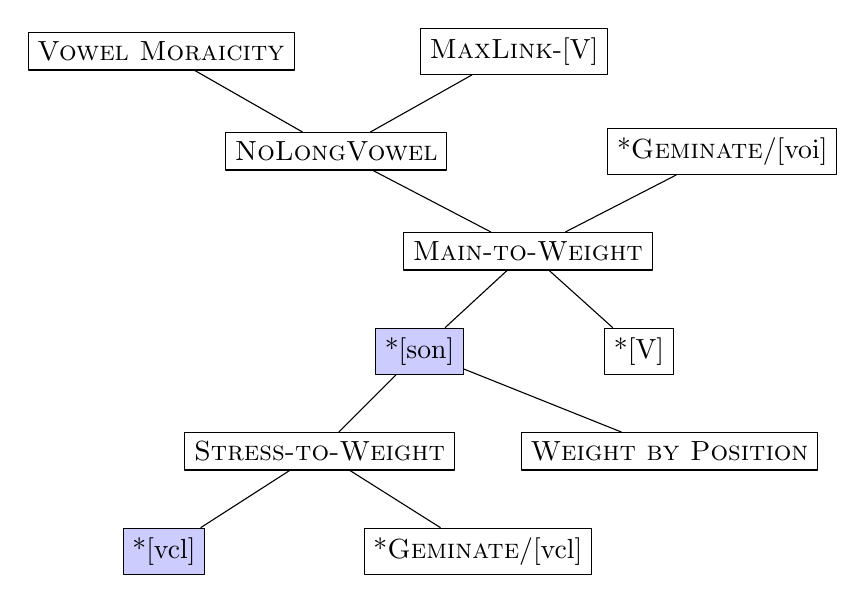
\begin{tikzpicture}[>=latex,line join=bevel,yscale=.5]
%%
\node (Max-m-V) at (194bp,378bp) [draw,rectangle] {\textsc{MaxLink}-\mo[V]};
  \node (Vowel Moraicity) at (67bp,378bp) [draw,rectangle] {\textsc{Vowel Moraicity}};
  \node (WbP) at (250bp,90bp) [draw,rectangle] {\textsc{Weight by Position}};
  \node (*m[vcl]) at (68bp,18bp) [draw,rectangle,fill=blue!20] {*\mo[vcl]};
  \node (MtW) at (199bp,234bp) [draw,rectangle] {\textsc{Main-to-Weight}};
  \node (*m-son) at (160bp,162bp) [draw,rectangle,fill=blue!20] {*\mo[son]};
  \node (*Geminate/son) at (269bp,306bp) [draw,rectangle] {*\textsc{Geminate}/[voi]};
  \node (StW) at (124bp,90bp) [draw,rectangle] {\textsc{Stress-to-Weight}};
  \node (*mm) at (239bp,162bp) [draw,rectangle] {*\mo[V]};
  \node (*Geminate/vcl) at (181bp,18bp) [draw,rectangle] {*\textsc{Geminate}/[vcl]};
  \node (NoLongVowel) at (130bp,306bp) [draw,rectangle] {\textsc{NoLongVowel}};
  \draw [] (*Geminate/son) -- (MtW);
  \draw [] (MtW) -- (*mm);
  \draw [] (Vowel Moraicity) -- (NoLongVowel);
  \draw [] (MtW) -- (*m-son);
  \draw [] (NoLongVowel) -- (MtW);
  \draw [] (*m-son) -- (WbP);
  \draw [] (*m-son) -- (StW);
  \draw [] (StW) -- (*Geminate/vcl);
  \draw [] (Max-m-V) -- (NoLongVowel);
  \draw [] (StW) -- (*m[vcl]);
%
\end{tikzpicture}
  \caption{Ranking for Latvian facts in line with \citet{bye08}}
  \label{fig:latvian-bdl}
\end{figure} While it demonstrates that a ranking consistent with all these conditions does exist, it also shows an undesirable consequence of trying to view obstruent gemination as a phonological process: it requires *\mo[sonorant] to dominate *\mo[voiceless obstruent] (highlighted boxes). This is because *\mo[sonorant] dominates \textsc{Stress\hyp to\hyp Weight} (which accounts for the lack of coerced weight of sonorant codas, and consequently tonal accents, under secondary stress), but *\mo[voiceless obstruent] has to be dominated by \textsc{Stress\hyp to\hyp Weight} for obstruent gemination to be possible.

This ranking goes against the standard approach according to which less sonorous segments cannot be preferred to more sonorous ones as moraic codas under coercion \citep{zec88:_sonor,ot,delacy2006}. This would appear to call for a \textsc{DepLink}\hyp based solution à~la \citet{moren01:_distin}. The constraint \textsc{DepLink}-\mo[sonorant] is freely rerankable, and so it can be ranked above *\mo[voiceless] to prohibit sonorant moraicity in unstressed syllables without jeopardizing the sonority\hyp based hierarchy. However, below in \cref{sec:inertn-textscd-mo} I show that the use of \textsc{DepLink}-\mo[V] in situations of this sort presents certain problems with faithfulness, because it cannot rule out preservation of underlying morae on sonorants in unstressed syllables.

In any case, perhaps a more fruitful approach to the Latvian data involves rejecting obstruent gemination as a phonological process altogether. I suggest that it can be viewed as a \emph{phonetic} correlate of stress. If we exclude obstruent gemination from the phonology, there is no need for \textsc{Stress\hyp to\hyp Weight} dominating *\mo[voiceless]: indeed we can uphold \posscite{bye08} suggestion that only main stress can be enhanced by qualitative alternations, and thus the problematic ranking disappears. However, it is clear that only deeper phonological analysis and further instrumental study can confirm or deny this suggestion.

In this section I considered some Latvian data presented by \citet{bye08} and analysed by them without recourse to mora enhancement. Although these data bear a certain resemblance to those found in Welsh, I have argued that closer attention to the Latvian system shows that its pattern does not necessarily provide a good parallel for Welsh. (I will consider an analysis of Welsh in terms of *\textsc{Geminate} constraints without the additional complications in \cref{sec:against-antig}.)

In any case, a similar approach to Welsh would require us to view the lengthening of consonants as a phonetic rather than as a phonological fact (\cf the discussion of length as a \enquote{correlate of stress} in Welsh in \cref{sec:real-stress-polysyll} above). Although such an account is feasible in principle, it runs into problems with Richness of the Base. Specifically, the contrast between short and long vowels in the context before \ipa{[n~l~r]} is clearly relevant to the phonology, since it has to do with lexical contrast. Even if this lexical contrast is implemented as one of vocalic rather than consonantal length, we still have no account of why only long vowels are found before segments such as \ipa{[b~d~ɡ]} and only short ones precede \ipa{[p~t~k]}: in \cref{cha:pembrokeshire-welsh} I assume that these restrictions are not accidental (but see below \cref{sec:concl-typol-impl} for an alternative approach). In this, Welsh crucially differs from Latvian, where the surface distribution of vowel length is quite free, and the problems with the rich base do not arise.

\paragraph{Gemination and moraicity}
\label{sec:gemination-moraicity}

The analysis of Latvian given in the preceding paragraph highlights an important (potential) distinction that we will need to take into account below. It shows that gemination (whether understood as multiple association or ambisyllabicity) \emph{must} be distinguished from moraicity \citep{selkirk90,ringen11:_gemin}. As \cref{fig:latvian-bdl} shows, the constraint against \enquote{geminate} (long) sonorants must dominate \textsc{Main\hyp to\hyp Weight}, as hypothesized by \citet{bye08}, but the constraint against moraic (not necessarily long) sonorants must be ranked lower than \textsc{Main\hyp to\hyp Weight} in order to produce a heavy stressed syllable under main stress; it follows that these are in fact \emph{different} constraints. I will discuss this distinction in more detail below (\cref{sec:against-antig}).

\subsubsection{Deriving laryngeal contrast}
\label{sec:deriv-laryng-contr}

In this section I consider a class of solutions which treat the laryngeal contrast as either epiphenomenal or somehow derived from a quantity contrast. If this were the case in Welsh, there would be no need for moraic enhancement, since all the vowel length facts would follow straightforwardly from the quantity\hyp based phonological surface representation. I will argue that adopting such a solution for Welsh still necessitates some device requiring that certain featural structures be associated with length, which is, in effect, equivalent to the moraic enhancement approach offered in \cref{sec:foot-intern-struct}.

\paragraph{High German: a purely quantitative system}
\label{sec:high-german}

The most straightforward type of a quantity\hyp based system only uses length to distinguish between classes of consonants, without enhancing it by some other means or transforming the quantitative system into a featurally based one in the phonological computation. Precisely such a system is found in Thurgovian High German \citep{kraehenmann01:_swiss_german,kraehenmann03:_quant_aleman,kraehenmann08:_durat_swiss_german}; as argued by \citet{seiler09:_sound}, this sort of contrast appears to be characteristic (at least historically) of many High German dialects (see also \citealt{lahiri04}).

In Thurgovian German, the contrast between \enquote{fortis} and \enquote{lenis} obstruents and sonorants is one of length (closure duration for stops, segment duration for fricatives and sonorants). There are also top-down conditions on syllabic structure, and in particular word minimality restrictions which cause vowel lengthening before singleton (\enquote{lenis}) obstruents in monosyllabic forms but not before certain consonant sequences or long (\enquote{fortis}) obstruents (see also \citealt{seiler05:_open_bernes_german} for a related interpretation of similar facts in Bernese German, although \citealt{ham01:_phonet} treats the Bernese pattern as open syllable shortening); examples are given in \ref{ex:thurgau-exx}.

\ex.\label{ex:thurgau-exx}\a.\a.\mbi{[ˈtːaːk]}`day'
\b.\mbi{[ˈtːakə]}`days'
\z.\b.\a.\mbi{[ˈafː]}`monkey'
\b.\mbi{[ˈafːə]}`monkeys'
\z.\b.\a.\mbi{[ˈpurk]}`castle'
\b.\mbi{[ˈpurkə]}`castles'

The Thurgovian fortis\hyp lenis contrast corresponds to the laryngeal contrast (\ie the [$\pm$voice] of traditional analyses and the [spread glottis]-based system of \citealt{iverson95,iverson99:_laryn_german,jessen02:_laryn_german,honeybone05}) of other German varieties. Rewritten in a more traditional transcription, the examples in \ref{ex:thurgau-exx} do indeed show a striking similarity to the Welsh alternation: \alternation{[ˈtaːɡ]}{[ˈtaɡə]}, \alternation{[ˈaf]}{[ˈafə]}. What makes the Thurgovian German a good \emph{comparandum} for Welsh is that the quantity contrast can be preserved in all prosodic positions, including absolute initial \citep{kraehenmann08:_durat_swiss_german}, which makes it quite similar to featural contrasts and quite unlike a moraicity distinction.

Another interesting consequence of the non\hyp existence of a laryngeal contrast in Thurgovian German is the fact that it is impossible (arguably for representational reasons) to have multiple types of sequences: the \enquote{laryngeal} contrast is always neutralized in sequences. As \citet{kraehenmann03:_quant_aleman} shows at length, two adjacent obstruents are always \enquote{lenis} on the surface; but a sequence of two lenis obstruents is, from the point of view of the laryngeal\fshyp quantitative contrast, indistinguishable from a fortis. This unification of lenis sequences with fortis consonants is extremely reminiscent of phonological provection in the Brythonic languages, and indeed in \cref{sec:leonais-breton} I discuss a very similar analysis of Breton by \citet{carlyle88:_breton}.

However, the Thurgovian German analysis cannot be directly transplanted to the Welsh data for a number of reasons. Most importantly, the Thurgovian contrast is primarily one of quantity not just phonologically but also phonetically. Welsh clearly contrasts its fortis and lenis consonants not just in terms of quantity, but also in terms of other features, and I presume that some account of these must also be given. This is especially true if we assume that lenis (\ie \enquote{short}) consonants in Welsh can in fact be long without neutralizing with fortis ones. One context where this happens in Welsh is in examples with a stressed schwa like \ipa{[ˈɬədan]} `wide'; if \posscite{awbery86:_pembr_welsh} dictum that consonants are long after a short stressed vowel applies in this case (\ie the word is \phonint{ˈɬədˑan} phonetically), then the fact that it does not change to *\ipa{[ˈɬətan]} demonstrates the independence of laryngeal contrast and quantity in Welsh. Unfortunately I have not found sources treating these issues specifically, so I let this stand as a falsifiable prediction.\footnote{Even if the stop in \ipa{[ˈɬədan]} turns out not to lengthen (\ie it is nonmoraic), this does not invalidate the proposals for foot structure made in\cref{sec:foot-intern-struct}. In this case, words like \ipa{[ˈɬədan]} are treated like Latvian \ipa{[ˈmizɑ]} `bark', at the cost of a violation of \textsc{FtBin}.}

Nevertheless, languages such as Thurgovian German are a good starting point, because they show very clearly that the connection between vowel length and laryngeal features of following consonants, which is also observed in Middle High German and in many modern dialects, is mediated, at least historically, not by the laryngeal features themselves but by the quantity of the consonant; for ample discussion of this issue with reference to German, see \citet{seiler09:_sound}.

\paragraph{Enhanced quantity contrast}
\label{sec:enhanc-qual-contr}

A more complicated case is found in languages where a phonological quantitative contrast is realized in concert with other phonetic features, including glottal state and manner. A typical feature of such systems is great variability in the realization of the contrast, especially with regard to obstruents: \enquote{fortis} obstruents are usually realized as relatively long consonants, most often without any voicing, and frequently accompanied by pre- and postaspiration, while \enquote{lenis} obstruents are shorter, often accompanied by some degree of voicing (although it is highly variable), and frequently spirantized. One area where such systems are frequent is Meso-America \citep[\cfm][]{campbell86:_meso_americ_linguis_area}, where they have been described, for instance, for Oto-Manguean languages, including many Zapotec languages (belonging to the Zapotecan group) and Mixtecan languages (another branch of Oto-Manguean), and Mixe (a member of the unrelated Mixe-Zoque family). Relevant literature includes \citet{jones77:_guelav_zapot,nellis80:_fortis_cajon_zapot,jaeger83,avelino01:_yalál_zapot,leander08:_acous_san_frans_ozolot_zapot} for Zapotec varieties, \citet{dicanio10:_ituny_trique} for the Mixtecan language Trique, and \citet{bickford85:_fortis_guich_mixe} for Mixe.

\citet{bye08} propose an account of Guelavía Zapotec \citep[citing][]{jones77:_guelav_zapot,gonzalez03} using *\textsc{Geminate} constraints. They claim that under main stress vowels are lengthened before lenis consonants, whereas when a stressed vowel is followed by a fortis consonant it is the consonant that becomes long, as in the following examples:

\ex.\a.\a.\mbi{[ˈra\emph{pː}a\textsuperscript{ʔ}]}`I have'
\b.\mbi{[ˈna\emph{ʃː}ɨŋ]}`it is sweet'
\z.\b.\a.\mbi{[ɾkwaˈβ\emph{eː}ðe]}`it is spicy'
\b.\mbi{[ˈɡ\emph{oː}zmɨ]}`sickle'

In parallel with their analysis of Latvian, \citet{bye08} treat the pattern as reflecting a ranking \dom{\textsc{Main-to-Weight}, *\textsc{Geminate/Lenis}}{\dom{\textsc{NoLongV}}{\textsc{*Geminate}}} which unfailingly enforces a bimoraic norm but prefers vowel lengthening to gemination when a lenis consonant is involved.

This analysis presupposes that the distinction between geminates and singletons and the contrast between fortis and lenis consonants are not in fact the same, \ie that \enquote{geminate lenes} and \enquote{singleton fortes} are conceivable representations that just happen not to surface because of the ranking. I would suggest that there is no compelling evidence to support this conclusion.

Phonetic studies on the relevant languages show that length is primary correlate of the fortis\fshyp lenis contrast (\citealp[see][]{jaeger83,avelino01:_yalál_zapot,leander08:_acous_san_frans_ozolot_zapot} on Zapotecan), and there are also certain phonological arguments, for instance based on inalterability. Nevertheless, the literature does contain proposals using in a fortis\fshyp lenis contrast orthogonal to length. In particular, \citet{nellis80:_fortis_cajon_zapot} draw attention to the variable realization of that contrast, in particular to the spirantization and voicing that frequently accompany lenis obstruents, which they treat as phonological. It must be noted, however, that such variation in manner and\fshyp or voicing is quite common in languages with small inventories that do not utilize these contrasts in their phonology \citep{lorentz07:_privat}, \ie the very variability that \citet{nellis80:_fortis_cajon_zapot} claim as an argument for the phonological relevance of a featural contrast can be taken as an argument \emph{against} the presence of a contrast. Moreover, the careful phonetic study of San Martín Itunyoso Trique by \citet{dicanio10:_ituny_trique} shows that \enquote{voicing} and \enquote{spirantization} (as well as aspiration characteristic of fortis obstruents) are best understood as more or less automatic concomitants of the realization of what is phonologically a quantity contrast; it seems plausible that a similar argument could be made for Guelavía Zapotec.

It is also not a given that \citet{bye08} are correct in treating the lengthening of vowels and consonants as described by \citet{jones77:_guelav_zapot} as reflecting the manipulation of moraicity by the phonological computation. For instance, \citet{jones77:_guelav_zapot} claim that Guelavía Zapotec fortis consonants are also lengthened word\hyp finally, even if the preceding vowel is not stressed:

\ex.\a.\mbi{[ˈkuʂːaʂː]}`magpie'
\b.\mbi{[ˈβelːakʰː]}`how much'

Rather than assuming a phrase\hyp final phonological process of mora addition, it seems better to treat this phenomenon as an instance of phonetic lengthening at a prosodic boundary \citep[à~la][]{wightman92:_segmen,fougeron,cho05:_prosod}. This means, however, that length in transcription does not necessarily correspond to phonological length; consequently, it does not follow from the transcription that the lengthening of vowels and\fshyp or consonants in the context of stress is also necessarily phonological. \citet{avelino01:_yalál_zapot} reaches a similar conclusion for Yalálag Zapotec. In particular, he finds that stress\hyp driven lengthening only happens before lenis \emph{obstruents} (\ie that lenis sonorants do not trigger lengthening), and that it affects both the vowel and the prevocalic consonant (which is unusual if the relevant process is adding a mora to the vowel). His conclusion is that lengthening of stressed vowels in Yalálag Zapotec is phonetic, and is not the result of a process that assigns two morae to stressed vowels before all lenis consonants, \ie it is just a correlate of stress.

Of course it is not possible to apply these findings uncritically to Guelavía Zapotec. Nevertheless, I suggest that, on balance, it appears that systems such as those found in Otomanguean languages do not require an account that separates gemination from the contrast between fortes and lenes. Thus, even if the vowel lengthening under stress is a phonological phenomenon, it appears that *\textsc{Geminate} constraints are not needed to account for the Guelavía Zapotec facts, since the length of fortes comes from the lexicon.

In other words, from a phonological perspective languages such as Guelavía Zapotec are not significantly different from systems such as those found in High German; the difference is in the phonetic realization of the contrast. While High German speakers mostly use duration to signal it, Zapotec speakers command a wider variety of (at least partially controlled) realizations; yet this difference may be of no consequence phonologically.

In the next section I consider a language where laryngeal contrast on the surface clearly cross\hyp cuts quantity, but which has nevertheless been analysed in terms of the former being derived from the latter. Incidentally, the variety in question is a Breton dialect.


\subsubsection{Léonais Breton}
\label{sec:leonais-breton}

In this section I consider \posscite{carlyle88:_breton} treatment of Léonais Breton (specifically the dialect of Lanhouarneau), which demonstrates a pattern of interactions between vowel length, consonant length, and laryngeal features that is similar to Welsh and to other Breton dialects (although, as we saw in \cref{sec:distr-vowel-length}, not in the dialect of Bothoa); the patterns are obviously related historically, see also \citet{falchun,lheb,histbreton,ternes11:_neubr}.

\paragraph{The data and \posscite{carlyle88:_breton} analysis}
\label{sec:data-possc-analys}

The pattern in Léonais Breton is extremely similar to that seen in Welsh, with the addition of final devoicing (and pre\hyp sonorant voicing). All consonants are assumed to be either lenis (short) or fortis (long).\footnote{Note that this sense of \enquote{fortis} and \enquote{lenis} is different from that used in some previous paragraphs as a cover term for [voiceless] and/or [spread glottis] à~la \citet{kohler84:_phonet}.} Stressed vowels are long before the former and short before the latter. In terms of voicing, fortis obstruents are almost always voiceless; lenis obstruents are voiced word-medially and voiceless word-finally. Word-final obstruents are always short.

\ex.Fortis obstruents
\a.Word-medial position
\a.\twe{[ˈskotːa]}{skaotañ}{to burn}
\b.\twe{[ˈbresːa]}{bresañ}{to shuffle one's feet}
\z.\b.Word-final position: degemination (and devoicing) with vowel lengthening
\a.\twe{[ˈskoːt]}{skaota}{(s)he burns}
\b.\twe{[ˈbreːs]}{bresa}{(s)he shuffles his (her) feet}

\ex.Lenis obstruents
\a.Word-medial position
\a.\twe{[ˈdiːbu]}{dibroù}{saddles}
\b.\twe{[ˈøːɡys]}{heugus}{disgusting}
\z.\b.Word-final position: devoicing, vowel lengthening intact
\a.\twe{[ˈdiːp]}{dibr}{saddle}
\b.\twe{[ˈøːk]}{heug}{disgust}

\ex.Sonorants
\a.Fortis sonorants
\a.Word-medial position\\
\twe{[ˈkolːu]}{kolloù}{losses}
\b.Word-final position: preservation in stressed syllables\\
\twe{[ˈkolː]}{koll}{loss}
\z.\b.Lenis sonorants: preceded by long vowels
\a.Word-medial position\\
\twe{[ˈpaːlu]}{palvoù}{palms}
\b.Word-final position\\
\twe{[ˈpaːl]}{palv}{palm}

Word-initially, \citet{carlyle88:_breton} claims that there is no underlying length contrast in sonorants, but that phonetically they may or may not be lengthened: \ipa{[ˈl(ː)oːar]} `moon' (\emph{loar}). Stops are said to be predictably fortis in word-initial position, although \citet{carlyle88:_breton} did not conduct measurements; she refers to \posscite{falchun} description, saying that her auditory impressions are broadly in agreement with his data. \citet[pp.~63--65]{falchun} does discuss initial obstruents, but only in a phrasal context; no data comparable to \posscite{kraehenmann03:_quant_aleman} for phrase-initial obstruents are available.

\citet{carlyle88:_breton} proposes that underlyingly Léonais Breton contrasts long and short obstruents and sonorants, but does not distinguish between voiced and voiceless obstruents. She proposes that rules governing the quantity of vowels operate at a point when these representations have not been converted into those with laryngeal features. \citet{carlyle88:_breton} suggests the following rule ordering:

\begin{enumerate*}
\item Word-final obstruent geminates are simplified to singletons;\footnote{The actual mechanism proposed by \citet{carlyle88:_breton} is more complex, but this need not concern us here.}
\item Stressed vowels are lengthened if possible (\ie unless followed by a long consonant or a consonant cluster);
\item Redundancy rules apply:
\begin{itemize*}
\item All word-final [$-$sonorant] segments become [$-$voice];\footnote{\citet{carlyle88:_breton} does not really discuss pre-sonorant voicing (apart from some brief remarks on p.~31).}
\item All [$-$sonorant] segments linked to more than one skeletal position become [$-$voice];
\item All other obstruents are [+voice].
\end{itemize*}
\item Word-initial consonants are lengthened (obligatorily in the case of obstruents, optionally in the case of sonorants), except in contexts for lenition.
\end{enumerate*}

The derivation up to the application of redundancy rules provides an elegant way of unifying vowel quantity and consonant quality, and specifically the connection between short stressed vowels and voiceless obstruents: both appear in the presence of more than one consonantal node. This approach also provides a simple account of what I call \enquote{morphological provection} in \cref{sec:morph-induc-prov}, \ie the devoicing of obstruents accompanied by the shortening of vowels. While Bothoa Breton as analysed in \cref{cha:bothoa-breton} requires that the provection\hyp inducing morpheme consist of both a floating \fea{C-lar}{vcl} feature (to produce segmental changes) and a mora (to produce prosodic alternations), \citet{carlyle88:_breton} is able to analyse it in terms of an empty segmental position associated with the suffix: it achieves both gemination of the stem\hyp final consonant (which blocks vowel lengthening) and devoicing (via the redundancy rule).

\paragraph{Aside: provection in Léonais}
\label{sec:asid-prov-leon}

Finally, although \citet{carlyle88:_breton} does not discuss these issues in detail, the redundancy rule which assigns \ipa{[$-$voice]} to adjacent obstruents takes care of phonological provection, \ie the prohibition against adjacent voiced obstruents. It seems that this rule applies in Léonais Breton as well, see especially \citet{falchun38:_recher,falchun}. \citet{carlyle88:_breton} does give forms which seem to show that it does not always apply, but they all implicate the segment \ipa{[v]}, and more specifically the ordinal numeral suffix \suff{ved} (cognate with Welsh \emph{-fed}, see \cref{sec:consonant-sequences-1}), as in the following examples (I leave \citeauthor{carlyle88:_breton}'s transcription unchanged, but add stress for clarity):\footnote{In Bothoa Breton, the suffix is \suff{əɡ}, so it cannot be used to provide evidence for or against provection.}

\ex.\label{ex:leonais-no-provection}\a.\twe{[ˈhwe\emph{xv}et]}{c'hwec'hvet}{sixth}
\b.\twe{[ˈde\emph{ɡv}et]}{degvet}{tenth}
\b.\twe{[triˈze\emph{ɡv}et]}{trezegvet}{thirteenth}

However, there is good evidence that the words in \cref{ex:leonais-no-provection} do not represent a true counterexample, because \ipa{[v]} in Léonais Breton functions as a sonorant rather than an obstruent. This is related to the existence of a fourth third labial continuant alongside \ipa{[f]}, \ipa{[v]}, and \ipa{[w]}. Found in many northern dialects, it is usually described as \enquote{half-voiced} (Carlyle 1988) or a voiced fricative with more noise than \ipa{[v]} (\cf \citealt[p.~366]{plougrescant}: \enquote{labiodental, lenis [and] more energetically puffed than \ipa{[v]}, [\ldots] a voiceless \ipa{[v]} which is well aspirated, and might therefore be written \ipa{[v̥h]}}); this segment is found in Léonais dialects such as Lanhouarneau \citep{carlyle88:_breton}, Le Bourg Blanc \citep{falchun}, Saint-Pol-de-Léon \citep{st-pol-de-leon}, and Berrien \citep{ploneis}, and in Trégorrois varieties such as Plougrescant \citep{plougrescant,le78:_le_ploug} and Pleubian \citep{le96:_mutat_pleub_côtes_nord}. I am going to write it \ipa{[f̬]}. In many of these dialects, there is evidence that it is this fricative \ipa{[f̬]} that is the laryngeally specified counterpart of \ipa{[f]}, while \ipa{[v]} stands outside the laryngeal contrast.

In Lanhouarneau, the evidence comes from final devoicing (or rather final degemination, as \citealt{carlyle88:_breton} treats it). Here, word\hyp final \ipa{[f]} alternates with \ipa{[f̬]} rather than \ipa{[v]} (the examples and analysis are \citeauthor{carlyle88:_breton}'s):

\ex.\a.\twe{[ˈkoːf]}{kof}{stomach}
\b.\twe{[ˈkoːf̬u]}{kofoù}{stomachs}
\b.*\mbi{[ˈkoːvu]}

In turn, word\hyp medial \ipa{[v]} alternates with \ipa{[o]}:

\ex.\label{ex:leonais-vocalization}\a.\a.\twe{[ˈbeːo]}{bev}{alive}
\b.\twe{[ˈbeːva]}{bevañ}{to live}
\z.\b.\a.\twe{[ˈbeːro]}{berv}{boiling}
\b.\twe{[ˈbervet]}{bervet}{boiled}

Since non\hyp alternating \ipa{[o]} also exists (\ipa{[ˈɡoːro]} `to milk', \ipa{[ɡoˈroːet]} `milked' (\emph{goro}, \emph{goroet})), it is best to treat the alternations in \cref{ex:leonais-vocalization} as the vocalization of underlying \ipa{[v]}.\footnote{Typologically, this vocalization is quite similar to that found with word-final sonorants in languages such as Serbian \citep[\egm][]{moren-serbian}.}

More evidence is available from other dialects. For instance, in Plougrescant word-initial voiced fricatives become voiceless when preceded by another obstruent (examples from \citeauthor{le78:_le_ploug} \cite*{le78:_le_ploug}, p.~148):

\ex.\a.\a.\twe{[f̬alː]}{fall}{bad}
\b.\twe{[ə map ˈfalː]}{ur mab fall}{a bad boy}
\z.\b.\a.\twe{[ˈzeː]}{se}{this}
\b.\twe{[ˈn aːbit se]}{an abid-se}{this suit}
\z.\b.\a.\twe{[ˈʒarl]}{Jarl}{Charles}
\b.\twe{[taːt ˈʃarl]}{tad Jarl}{Charles' father}

It would seem that this phenomenon is best described in terms similar to provection, \ie the addition of a [voiceless] feature to a doubly linked C\hyp laryngeal node spanning the word boundary. Crucially, this phenomenon is not described for \ipa{[v]}, which does appear in word\hyp initial position (albeit rarely). This can be explained if it is a sonorant and thus lacks a laryngeal specification.

Finally, the status of \ipa{[v]} as a sonorant is confirmed in Plougrescant Breton by the fact that it can precede a sonorant in word\hyp final position. In general, rising\hyp sonority sequences are disallowed word\hyp finally in that dialect, and they are repaired by deletion of the sonorant (all examples from \citeauthor{le78:_le_ploug} \cite*{le78:_le_ploug}; I write final obstruents as voiced following the source, although in practice they are also voiceless):

\ex.\label{ex:plougrescant-rising-sonority}\a.\a.\twe{[ˈmɛst]}{mestr}{master}
\b.\twe{[ˈmɛstro]}{mestroù}{masters}
\z.\b.\a.\twe{[ˈdub]}{doubl}{lining}
\b.\twe{[ˈdublã]}{doublañ}{to line}
\z.\b.\a.\twe{[ˈɡɔːb]}{gobr}{wages}
\b.\twe{[ˈɡɔbrɛst]}{gobr-eost}{contract for the harvest season}

However, \ipa{[v]}\endash sonorant sequences are allowed:

\ex.\a.\twe{[ˈæ̃vn]}{evn}{bird}
\b.\twe{[ˈkwævr]}{kouevr}{copper}

This further confirms that \ipa{[v]}, unlike \ipa{[f̬]}, is treated as a high\hyp sonority segment in Breton, and thus provection is not expected to apply in \cref{ex:leonais-no-provection}.\footnote{As \citet{carlyle88:_breton} herself notes, an underlying \ipa{[v]} can in fact be devoiced to \ipa{[f]} in word\hyp final position, but this happens in a restricted morphological environment\dash the 3sg person singular present of verbs\dash as in \ipa{[ˈliːf]} `((s)he) colours' from underlying \ipa{/liv/}. This ambiguous behaviour is of course not uncommon for \ipa{[v]} (with perhaps the most celebrated example being Russian; \eg \citealt{hayes84:_russian,kiparsky85:_some_lexic_phonol,padgett-vproblem}), but in any case I do not pursue these issues here for reasons of focus}

\paragraph{Issues with \posscite{carlyle88:_breton} analysis}
\label{sec:issues-with-analysis}

\posscite{carlyle88:_breton} analysis has a number of attractive properties, accounting for the interaction of vowel length and consonant quality, as well as morphological and phonological provection. Nevertheless, I suggest that it is neither quite workable for Léonais Breton (especially in an OT framework) nor adaptable to the Welsh facts, despite their close similarity to the Breton ones.

One problem with the approach used by \citet{carlyle88:_breton} is her treatment of initial strengthening. Recall that she proposes a rule of word\hyp initial gemination that applies after the redundancy rules have converted the length contrast into a laryngeal one.

This creates an opaque derivation (and a non\hyp vacuous Duke-of-York gambit). On the surface, voiced and voiceless obstruents contrast word\hyp initially: \ipa{[ˈɡleːp]} `wet' (\emph{gleb}), \ipa{[ˈkluːar]} `warm' (\emph{klouar}). However, \citet{carlyle88:_breton} analyses these as underlying \ipa{/klep/} and \ipa{/kkluar/}, respectively: the redundancy rules convert these into intermediate \ipa{/ɡlep/} and \ipa{/kluar/}, and then initial strengthening restores the gemination in the latter case: \ipa{[ˈɡːleːp]}, \ipa{[kːluːar]}.

The evidence for this analysis comes from the lenition mutation. Normally, it is described as voicing of voiceless stops and spirantization of voiced ones (\cf \cref{sec:lenition} for Bothoa). However, in Léonais Breton, if the laryngeal contrast in initial position is treated as a quantity distinction, lenition can be described as \enquote{degemination, with spirantization of singleton stops}. The process is illustrated by the lenition-inducing clitic \ipa{[e]} `his' and its contrast with \ipa{[e]} `her', which does not cause this mutation, instead causing spirantization.

\ex.\a.Sonorants: degemination
\a.\twe{[ˈl(ː)øːe]}{leue}{calf}
\b.\twe{[e ˈløːe]}{e leue}{his calf}
\b.\twe{[e ˈlːøːe]}{he leue}{her calf}
\z.\b.Voiceless stops: voicing as degemination
\a.\twe{[ˈpːaːs]}{paz}{cough}
\b.\label{ex:e-baz}\twe{[e ˈbaːs]}{e baz}{his cough}
\b.\twe{[e ˈfːaːs]}{he faz}{her cough}\footnote{\citet[p.~53]{carlyle88:_breton} gives this form as \ipa{[e ˈvːaːs]}, but elsewhere (p.~71) she discusses spirantization as changing voiceless stops into voiceless fricatives, with further voicing possible but optional, as shown here.}
\b.\mbi{[e ˈf̬ːaːs]}
\z.\b.Voiced stops: geminates not derived by mutation
\a.\twe{[ˈbːaːs]}{bazh}{stick}
\b.\twe{[e ˈvaːs]}{e vazh}{his stick}
\b.\label{ex:e-bbaz}\twe{[e ˈbːaːs]}{he bazh}{her stick}

The crucial contrast is that between \ref{ex:e-baz} and \ref{ex:e-bbaz}. In \cref{ex:e-bbaz}, the initial consonant is treated as underlyingly single; its gemination is due to the general rule enforcing the fortisness of all initial consonants, which applies \emph{after} the quantity\hyp based representations have been converted into voicing\hyp based ones. Conversely, in \cref{ex:e-baz} the degemination is derived: underlyingly, the consonant is long, the lenition\hyp causing clitic forces a shortening; after which the quantity\hyp to\hyp voice conversion applies to create a voiced stop.

While this account does provide an apparently elegant unification of voicing and quantity facts, it crucially relies on an entirely unmotivated stipulation. Specifically, word\hyp initial gemination is inert just in case lenition has applied before it. This explains the contrast before the short \ipa{[v]} in \ipa{[e ˈvaːs]} `his stick', which is derived by lenition, and the long \ipa{[f̬]} in \ipa{[e ˈf̬ːaːs]} `her cough', where the mutation does not lead to degemination.

Note that the difference between lenition and spirantization cannot be saved via rule ordering or similar mechanisms such as stratal computation. Specifically, if the voicing of stops seen in lenition is to be derived by their degemination (as Carlyle implies), lenition \emph{must} precede the redundancy rules assigning [+voice] to single obstruents. On the other hand, the redundancy rule must precede initial gemination, because otherwise the latter would neutralize the underlying contrast between fortes and lenes. Spirantization, on the other hand, apparently has to follow at least the redundancy rules, because it is able to produce voiced fortes (\cf Carlyle 1988, p.~72).

Thus, lenition must be separated from initial gemination by at least one other rule, namely the redundancy rules. Crucially, since the redundancy rules make reference to word\hyp final position, they should be available at the word level.\footnote{\citet{carlyle88:_breton} does not discuss the phonotactics and especially alternations in sufficient detail to evaluate the hypothesis that the redundancy rules refer to the coda, so I take the analysis at face value. Given the syllable structure rules discussed by \citet[ch.~3]{carlyle88:_breton}, an obstruent can only be parsed in a word\hyp internal coda if it is followed by another obstruent, in which case it will always fall under the purview of the redundancy rule assigning [$-$voice] to adjacent obstruents.} Initial gemination, on the other hand, would appear to be a postlexical rule, in particular given its optional status \citep[\egm][]{kiparsky85:_some_lexic_phonol}.\footnote{Again, I take the descriptions of initial gemination by \citet{falchun} and \citet{carlyle88:_breton} at face value and accept the assumption that it is in fact a phonological rule (although other descriptions of Léonais such as those by \citealt{sommerfelt62:_notes_dourd_plouez_finis,st-pol-de-leon} do not note it). I would suggest that the relationship between word\hyp medial long consonants in stressed syllables and long consonants word\hyp initially is worthy of targeted empirical study, but given that the analysis of Léonais is not the focus of this thesis, I refrain from further speculation on this point here.} Making sure that word\hyp initial gemination does not apply to lenited consonants requires some sort of (probably diacritical) marking to persist through several derivational levels, and I would suggest this is a sufficiently severe violation of many assumptions regarding locality and modularity (usually treated under the rubric of \enquote{bracket erasure}) that the analysis becomes suspect. Yet the analysis of lenition as degemination is absolutely crucial to undermining the distinctive status of laryngeal features in Lanhouarneau Breton, because it forms the cornerstone of the edifice that is the derivation of laryngeal contrast from quantity in initial position.

Another issue with \posscite{carlyle88:_breton} analysis also has to do with the supposed dependence of featural structure on quantity. In Lanhouarneau Breton, the fortis\fshyp lenis contrast is relevant for all obstruents, so laryngeal oppositions can be derived from it with no loss of information. In the case of sonorants, the fortis\hyp lenis (or length) contrast also exists, manifesting itself as length (and interacting with vowel quantity in a way parallel to that of obstruents). However, there are three sonorants in Léonais Breton that \enquote{are without an underlying lenis counterpart} \citep[p.~34]{carlyle88:_breton}: these are \ipa{[m]}, \ipa{[ɲ]}, and \ipa{[ʎ]}.\footnote{Recall that Welsh has a parallel in the behaviour of \ipa{[m]} and \ipa{[ŋ]}.} These segments are always long, and thus preceded by a short stressed vowel:

\ex.\a.\a.\twe{[ˈtomː]}{tomm}{hot}
\b.\twe{[ˈbremːã]}{bremañ}{now}
\z.\b.\a.\twe{[ˈsteɲː]}{stenn}{stiff}
\b.\twe{[ˈbaɲːel]}{bannier}{banner}
\z.\b.\a.\twe{[ˈsaʎː]}{sailh}{bucket}
\b.\twe{[ˈtryʎːa]}{truilhañ}{to dust}

\citet{carlyle88:_breton} seems to treat this fact as an input generalization: note the word \enquote{underlying} in her formulation. However, this is clearly unacceptable in an OT context. The fact that fortis and lenis sonorants are phonologically distinct (in that they exhibit different behaviour with respect to stressed vowel length) confirms that quantity and featural content \emph{are} represented differently in the phonology, and therefore any analysis must take into account the behaviour of all combinations of quantity and quality provided by the rich base. The fact that \ipa{[m~ɲ~ʎ]} can only be long following a stressed vowel cannot be ascribed solely to the fact that they are long in the input representation: the computation must enforce this length in some manner.

The fortis sonorants also pose a problem for \posscite{carlyle88:_breton} analysis as presented. She assumes that word\hyp final extrametricality affects all consonants (or consonant sequences) which form licit onsets \citep[\cfm][]{borowsky86:_topic_englis,ito86:_syllab}. Since both fortis and lenis obstruents are possible as onsets, they become extrametrical in word\hyp final position. Therefore, stressed vowels are always lengthened in monosyllables before obstruents, leading to alternations such as \alternation{[ˈskotːa]}{[ˈskoːt]} `\alternation{to burn}{(s)he burns}'. In the case of sonorants which contrast for length, the distinction is preserved:

\ex.\a.\twe{[ˈjeːn]}{yen}{cold}
\b.\twe{[ˈjenː]}{genn}{wedge}

\citet{carlyle88:_breton} argues that only lenis sonorants become extrametrical, because there is no contrast in sonorant length word\hyp initially, and thus \ipa{[nː]} is an impossible onset; this lack of extrametricality blocks vowel lengthening in \ipa{[ˈjenː]}. However, she does not consider the fortis sonorants. The lack of vowel lengthening before \ipa{[ɲ]} and \ipa{[ʎ]} is in principle amenable to \posscite{carlyle88:_breton} account, since they are impossible word\hyp initially. However, \ipa{[m]} is very much a possible onset, despite being fortis. Thus it would appear that \citet{carlyle88:_breton} predicts it to become extrametrical in word\hyp final position and fail to block vowel lengthening, hence counterfactual *\ipa{[toːm]} `warm' from underlying \ipa{/ttomm/}, in parallel to \ipa{[ˈskoːt]} `(s)he burns' from underlying \ipa{/skott/}. I conclude that simply assuming that \ipa{[m~ɲ~ʎ]} are underlyingly fortis is not sufficient to account fully for the facts of Léonais Breton.\footnote{I also note in passing that \posscite{carlyle88:_breton} approach to final extrametricality is apparently unable to cope with the facts of Welsh. Recall that in Welsh voiceless stops block vowel lengthening in both word\hyp medial and word\hyp final positions: \ipa{[ˈsopas]} `porridge', \ipa{[ˈkrut]} `boy'. This could only be the case in \posscite{carlyle88:_breton} system if they were impossible onsets, which is clearly incorrect. In addition, the voiceless fricatives \ipa{[f~θ~χ]} in Welsh do not block vowel lengthening, meaning they are \enquote{lenis}, which at the very least complicates the redundancy rules by making it necessary to refer to manner and not just laryngeal specification.}

Thus, even in a language with what appears to be independent evidence for the derivation of laryngeal contrasts from a quantity distinction in consonants, where the facts closely parallel those of Welsh, a purely representational solution does not appear to be feasible: at least \emph{some} computational device \emph{must} be present to ensure that consonants of a certain quality are necessarily geminated following a stressed nucleus, in preference to vowel lengthening. Since the evidence tying the surface laryngeal contrast to a surface distinction (\ie the analysis of lenition as degemination) is highly suspect, it would appear that an analysis along the lines of \cref{cha:pembrokeshire-welsh}, which takes the quality contrast to be underlying and deriving surface length of both obstruents and sonorants from quantity and prosodic structure, is preferable to the one presented by \citet{carlyle88:_breton}.

\paragraph{A radical substance-free alternative}
\label{sec:radic-subst-free}

It would appear that the Breton facts could in principle be amenable to a treatment in terms of quantity under a very expansionist conception of the phonetics\endash phonology interface. Specifically, we could assume that neither initial gemination nor the redundancy rules are part of the phonology, \ie that the surface phonological representation in Breton is purely quantity\hyp based like in Thurgovian German (\cref{sec:high-german}). In this case, there is no opacity and no violation of modularity, while the quantity facts follow all but automatically from the presence of a syllable coda (\cf Carlyle 1988, ch.~3 for a discussion of syllabification).

However, this approach requires an ever more radical substance\hyp free approach to representation than that espoused in the present thesis. In particular, it requires the phonetics\hyp phonology interface to make what is apparently a categorical distinction between two types of realization for singleton obstruents, \ie the categorically voiced type in onset position and voiceless (or underspecified) word\hyp finally; I argued in \cref{sec:interf-as-interpr} that this is perhaps not a desirable property of the interface.

Moreover, even if this solution is viable in principle, it does not help with the problem of the fortis sonorants \ipa{[m~ɲ~ʎ]}: given Richness of the Base, the computation still has to make sure that these always surface as long (except when they are word\hyp initial of follow a consonant). I would thus suggest that it is not feasible to fully explain the interaction between vowel length and consonant quality without recourse to some sort of computational device ensuring the surface length of consonants which possess certain features, even if a highly abstract mechanism is used to derive consonant quality from quantity. In the next section I will argue that the moraic enhancement approach used in \cref{sec:foot-intern-struct} is superior for this purpose than one based on antigemination constraints.

\subsubsection{Against antigemination}
\label{sec:against-antig}

So far I have argued that consonant quantity in Welsh is both manipulated by the phonological computation (\ie there is a difference between moraic and nonmoraic consonants in surface representations in this language) and distinct from featural content (\ie that both \enquote{voiced} and \enquote{voiceless} obstruents, for example, can be both \enquote{short} and \enquote{long}).\footnote{I would suggest that the analysis of Welsh should be adaptable to Breton dialects showing similar patterns, such as that of Lanhouarneau, but I leave this for future work.}

\begin{table}[htp]
  \centering
  \begin{tabular}{lcc}
    \toprule
    & \multicolumn{2}{c}{Preceding vowel length} \\
    \cmidrule{2-3}
    Consonants & Medially & Finally \\
    \midrule
    \ipa{[p t k]} & \multicolumn{2}{c}{Short} \\
    \ipa{[b d ɡ]} & \multicolumn{2}{c}{Long} \\
    \ipa{[v ð]} & \multicolumn{2}{c}{Long} \\
    \ipa{[f θ χ]} & \multicolumn{2}{c}{Long} \\
    \ipa{[s ʃ ɬ]} & Short & Long \\
    \ipa{[m ŋ]} & \multicolumn{2}{c}{Short} \\
    \ipa{[n l r]} & \multicolumn{2}{c}{Lexical} \\
    \ipa{[h]} & \multicolumn{2}{c}{Not found} \\
    \bottomrule
  \end{tabular}
  \caption{Vowel length before consonants in Pembrokeshire Welsh}
  \label{tab:vowel-length-disc-chapter}
\end{table}

\begin{table}[htp]
  \centering
  \subtop[Word-medial position]{%
  \begin{tabular}{>{\ipafont}l>{\ipafont}l>{\ipafont}c>{\ipafont}c}
    \toprule
                           &       & \multicolumn{2}{c}{Input length} \\
    \cmidrule{3-4}
    Segments               & Input & \ipa{V}   & \ipa{Vː}             \\
    \midrule
    \multirow{2}{*}{p t k} & t     & Vtˑ\gc    & Vtˑ\gc               \\
                           & t\smo & Vtˑ       & Vtˑ\gc               \\
    \midrule
    \multirow{2}{*}{b d ɡ} & d     & Vːd\gc    & Vːd                  \\
                           & d\smo & Vːd\gc    & Vːd\gc               \\
    \midrule
    \multirow{2}{*}{s~ʃ~ɬ} & s     & Vsˑ\gc    & Vsˑ\gc               \\
                           & s\smo & Vsˑ       & Vsˑ\gc               \\
    \midrule
    \multirow{2}{*}{f~θ~χ} & θ     & Vːθ\gc    & Vːθ                  \\
                           & θ\smo & Vːθ\gc    & Vːθ\gc               \\
    \midrule
    \multirow{2}{*}{v~ð}   & ð     & Vːð\gc    & Vːð                  \\
                           & ð\smo & Vːð\gc    & Vːð\gc               \\
    \midrule
    \multirow{2}{*}{m~ŋ}   & m     & Vmˑ\gc    & Vmˑ\gc               \\
                           & m\smo & Vmˑ       & Vmˑ\gc               \\
    \midrule
    \multirow{2}{*}{n~l~r} & n     & Vːn\gc    & Vːn                  \\
                           & n\smo & Vnˑ       & ?                    \\
    \midrule
    \multirow{2}{*}{u i}   & i     & Vi\smo\gc & Vi\smo\gc            \\
                           & i\smo & Vi\smo    & Vi\smo\gc            \\
    \bottomrule
  \end{tabular}}\hspace{3em}
  \subtop[Word-final position]{%
    \begin{tabular}{>{\ipafont}l>{\ipafont}l>{\ipafont}c>{\ipafont}c}
    \toprule
                           &       & \multicolumn{2}{c}{Input length} \\
    \cmidrule{3-4}
    Segments               & Input & \ipa{V}   & \ipa{Vː}             \\
    \midrule
    \multirow{2}{*}{p t k} & t     & Vt\gc     & Vt\gc                \\
                           & t\smo & Vt        & Vt\gc                \\
    \midrule
    \multirow{2}{*}{b d ɡ} & d     & Vːd\gc    & Vːd                  \\
                           & d\smo & Vːd\gc    & Vːd\gc               \\
    \midrule
    \multirow{2}{*}{s~ʃ~ɬ} & s     & Vːs\gc    & Vːs                  \\
                           & s\smo & Vːs\gc    & Vːs\gc               \\
    \midrule
    \multirow{2}{*}{f~θ~χ} & θ     & Vːθ\gc    & Vːθ                  \\
                           & θ\smo & Vːθ\gc    & Vːθ\gc               \\
    \midrule
    \multirow{2}{*}{v~ð}   & ð     & Vːð\gc    & Vːð                  \\
                           & ð\smo & Vːð\gc    & Vːð\gc               \\
    \midrule
    \multirow{2}{*}{m~ŋ}   & m     & Vm\gc     & Vm\gc                \\
                           & m\smo & Vm        & Vm\gc                \\
    \midrule
    \multirow{2}{*}{n~l~r} & n     & Vːn\gc    & Vːn                  \\
                           & n\smo & Vn        & ?                    \\
    \midrule
    \multirow{2}{*}{u i}   & i     & Vi\smo\gc & Vi\smo\gc            \\
                           & i\smo & Vi\smo    & Vi\smo\gc            \\
    \bottomrule
  \end{tabular}}
  \caption{Vowel and consonant length in Pembrokeshire Welsh stressed syllables}
  \label{tab:pw-vowel-lengths}
\end{table}


In \cref{sec:foot-intern-struct} I suggested that the pattern of vowel and consonant length found in Welsh (repeated for reference in \cref{tab:vowel-length-disc-chapter,tab:pw-vowel-lengths}\footnote{\Cref{tab:pw-vowel-lengths} shows all possible inputs (\ie including those supplied by the rich base). Shading indicates unfaithful mappings. Note that I take the projection of morae (indicated as half\hyp length word\hyp medially and as lack of vowel lengthening word\hyp finally) to be unfaithful. The outcome for input \ipa{/Vːn\smo{}/} is not known, because both \ipa{[Vn(ˑ)]} with vowel shortening and \ipa{[Vːn]} with mora delinking from the consonant are licit on the surface, and I am not aware of any evidence that would allow us to choose between them.}) is due to a set of constraints of the form \textsc{Have}-\mo[F], which promote the moraicity of segments specified for the feature(s) [F]. These constraints are dominated by overall prosodic constraints (so that bimoraic syllables only appear in the head of the prosodic word and moraic segments only appear in the coda) and by faithfulness constraints (which prevents \textsc{Have}-\mo[F] constraints from being repaired by changing featural specification of the relevant segments), but, crucially, they dominate constraints militating against consonant moraicity, allowing the consonants to become moraic and thus block vowel lengthening.

\citet{bye08} suggest that such patterns may be derived from the interaction of the constraint \textsc{NoLongVowel} and *\textsc{Geminate} constraints requiring that certain consonants remain singletons. As discussed in \cref{sec:gemination-moraicity}, these constraints must be able to refer specifically to long consonants, rather than singleton segments in the coda projecting a mora. Since \citet{bye08} do not discuss the relationship between gemination and moraicity explicitly \citep[\cfm][]{ringen11:_gemin} but do assume that gemination is used in the relevant cases to satisfy the constraint \textsc{Main\hyp to\hyp Weight}, which promotes bimoraicity, I assume that their account requires the coda portions of geminates to acquire a mora via something like \enquote{weight by position} applying across the board.

I consider word\hyp medial and word\hyp final consonants separately. For reference, \cref{tab:vowel-length-disc-chapter} repeats the patterns of stressed vowel length before various singleton consonants in Pembrokeshire Welsh.


\paragraph{Word-medial position}
\label{sec:word-medial-position}

In word\hyp medial position, the situation in Welsh is sufficiently similar to the cases described by \citet{bye08}, so the analysis can be transplanted relatively easily. The necessary ranking is shown in \cref{fig:ranking-word-medial}.\footnote{The ranking in \cref{fig:ranking-word-medial} assumes that voiced obstruents and \ipa{[f~θ~χ]} become moraic following a stressed \ipa{[ə]}, \ie that the correct output for \ipa{/ɬədan/} `broad' is \ipa{[ˈɬə\smo{}d\smo{}a\smo{}n]} and not *\ipa{[ˈɬə\smo{}da\smo{}n]}; if the latter is the surface form, \textsc{Main\hyp to\hyp Weight} must be reranked below the relevant \textsc{*Geminate} constraints, which does not change the major point.} The most important point here is that the segments which allow lengthening of vowels are those for which the \textsc{*Geminate} constraint ranks above \textsc{NoLongVowel}, while those for which \textsc{*Geminate} is ranked below that constraint prefer gemination to vowel lengthening. Note that the ranking in \cref{fig:ranking-word-medial} does not include faithfulness constraints, which only play a rôle in the case of lexically long (or moraic) \ipa{[n~l~r]}; nevertheless, I include the constraint(s) \textsc{*Geminate}[n~l~r], because, as discussed in \cref{sec:foot-intern-struct}, stressed vowels are lengthened before underlyingly nonmoraic (short) \ipa{[n]}, \ipa{[l]}, and \ipa{[r]}.

\begin{figure}[htp]
  \centering

\begin{tikzpicture}[>=latex,line join=bevel,yscale=.7,xscale=.7]
%%
\node (*Geminate[n l r]) at (242bp,162bp) [draw,rectangle] {\textsc{*Geminate}\ipa{[n l r]}};
  \node (NoLongVowel) at (320bp,90bp) [draw,rectangle] {\textsc{NoLongVowel}};
  \node (*Geminate[m ng]) at (158bp,18bp) [draw,rectangle] {\textsc{*Geminate}\ipa{[m ŋ]}};
  \node (*Geminate[p t k]) at (481bp,18bp) [draw,rectangle] {\textsc{*Geminate}\ipa{[p t k]}};
  \node (*Geminate[ff th ch]) at (78bp,162bp) [draw,rectangle] {\textsc{*Geminate}\ipa{[f θ χ]}};
  \node (*Geminate[b d g]) at (398bp,162bp) [draw,rectangle] {\textsc{*Geminate}\ipa{[b d ɡ]}};
  \node (NoLongSchwa) at (245bp,234bp) [draw,rectangle] {*\ipa{[əː]}};
  \node (*Geminate[s sh ll]) at (320bp,18bp) [draw,rectangle] {\textsc{*Geminate}\ipa{[s ʃ ɬ]}};
  \node (MtW) at (395bp,234bp) [draw,rectangle] {\textsc{Main-to-Weight}};
  \node (*Geminate[f dd]) at (553bp,162bp) [draw,rectangle] {\textsc{*Geminate}\ipa{[v ð]}};
  \draw [] (NoLongVowel) -- (*Geminate[p t k]);
  \draw [] (*Geminate[ff th ch]) -- (NoLongVowel);
  \draw [] (NoLongVowel) -- (*Geminate[m ng]);
  \draw [] (*Geminate[b d g]) -- (NoLongVowel);
  \draw [] (*Geminate[n l r]) -- (NoLongVowel);
  \draw [] (NoLongSchwa) -- (*Geminate[f dd]);
  \draw [] (*Geminate[f dd]) -- (NoLongVowel);
  \draw [] (NoLongSchwa) -- (*Geminate[b d g]);
  \draw [] (MtW) -- (*Geminate[f dd]);
  \draw [] (NoLongSchwa) -- (*Geminate[ff th ch]);
  \draw [] (MtW) -- (*Geminate[b d g]);
  \draw [] (MtW) -- (*Geminate[n l r]);
  \draw [] (MtW) -- (*Geminate[ff th ch]);
  \draw [] (NoLongVowel) -- (*Geminate[s sh ll]);
  \draw [] (NoLongSchwa) -- (*Geminate[n l r]);
%
\end{tikzpicture}

  \caption{Ranking for Welsh with *\textsc{Geminate} constraints: word-medial position}
\label{fig:ranking-word-medial}
\end{figure}

In principle, the ranking in \cref{fig:ranking-word-medial} is unobjectionable in a substance\hyp free theory of phonology. It does, however, pose some awkward questions for approaches insisting on functionally motivated fixed rankings.

Taken in isolation, the fact that voiceless (\enquote{fortis}) stops are more prone to gemination than voiced (\enquote{lenis}) ones has a straightforward phonetic explanation: obstruent articulations are inimical to voicing, since they lead to a build-up of pressure in the supralaryngel region, making it difficult to maintain a sufficient transglottal pressure differential for vocal fold vibration, and longer articulations obviously strengthen this effect. As a consequence, voiceless geminates are typologically preferred to voiced ones \citep[\egm][]{hirose07,ohala:_turbul}. However, such functional considerations obviously cannot be the entire story: at least \emph{a priori}, it appears difficult to propose similar functional explanations for the difference between the segment classes \ipa{[f~θ~χ]} (which do not prefer gemination) and \ipa{[s~ʃ~ɬ]} (which do). Thus, a certain rôle for more abstract (\ie functionally arbitrary) phonological computation is more or less unavoidable.

The most serious problem, however, lies in the fact the approach sketched in \cref{fig:ranking-word-medial} faces the stringent\hyp violation issue, as does any analysis that attempts to single out \enquote{lenis} stops for \emph{non\hyp gemination}: under the present featural assumptions, \textsc{*Geminate}\ipa{[b~d~ɡ]} is also violated by geminate \ipa{[p~t~k]} because of the inclusion of featural structures (see the tableau in \ref{stringent-problem} on \cpageref{stringent-problem}).

I discuss the status of sonority and  moraic markedness hierarchies below in \cref{sec:role-sonority}. However, before doing this, I present further arguments undermining an approach based on \textsc{*Geminate} constraints.

\paragraph{Word-final position}
\label{sec:word-final-position}

Constraints against long consonants can be formulated in a variety of ways. One option is that espoused by authors such as \citet{selkirk90,ringen11:_gemin}, who suggest that geminates are represented as nodes on a separate timing tier associated to a single root node which organizes subsegmental features. Another option is to assume a single root tier and view geminates as being associated to more than one prosodic node, \ie as ambisyllabic consonants.

The latter interpretation is not well suited to the Welsh facts. If \textsc{*Geminate} constraints are to be responsible for vowel length in all positions, then they should be inert in final\hyp syllables: in a word like \ipa{[ˈkrut]} `boy', where the vowel is short, and thus the consonant should be a \enquote{geminate}, there is no second syllable node to dominate the consonant.\footnote{A possible solution would be an empty nucleus \citep[\egm][]{kaye90,segeral01,scheer04}, which would then assimilate the situation in word\hyp final syllables to that in penultima, but then some special account would be needed for the difference in the behaviour of \ipa{[s~ʃ~ɬ]} in word\hyp final and word\hyp medial position. In the absence of compelling evidence for an empty nucleus (\eg from tone; \cf \citealt{kohnlein11:_rule}), I do not pursue this analysis further.}

Therefore, a \textsc{*Geminate} solution must rely on a separate timing tier, where nodes do not stand in a one\hyp to\hyp one relation to bundles of subsegmental features. However, we still need some account of the fact that \ipa{[s~ʃ~ɬ]} do not lengthen when word\hyp final: contrast \ipa{[ˈpeːɬ]} `far' and \ipa{[ˈdiɬad]} `clothes'.

It is of course possible to postulate a brute\hyp force constraint banning long \ipa{[s~ʃ~ɬ]} word\hyp finally. However, in addition to lacking explanatory force, such a constraint is problematic in terms of locality, since it mentions three objects, two of which are not adjacent (\ie two timing nodes and the word boundary): in other words, it is highly suspect on architectural grounds (\cf \citeauthor{buckley09:_local}'s \citeyear{buckley09:_local} critique of constraints such as \textsc{Lapse-at-End}).

One possible solution involves extrametricality of the final geminate. Since complex codas are all but prohibited in Pembrokeshire Welsh, one half of the geminate has to be extrametrical, giving the representations in \ref{ex:crwt-pell-comparison}. If (as I assume) extrametricality is formalized as the adjunction of the final segment to a recursive projection of the prosodic word node, a crucial difference between the two types of representations that is not apparent in the word\hyp medial context is that the first half of a geminated consonant is final in a minimal word projection (shaded), but a single consonant after a stressed vowel is only final in a maximal word projection. Thus, we can motivate the exclusion of long \ipa{[s~ʃ~ɬ]} in word\hyp final position by a constraint banning these consonants at the right edge of minimal projections of words.

\ex.\label{ex:crwt-pell-comparison}Final consonants in Wd$^{0}$\\
\begin{tabular}{ll@{\hspace{2em}}ll}
a. & \ipa{[ˈɬok]} `sheepfold' & b. & \ipa{[ˈpeːɬ]} `far' \\
&
\begin{tikzpicture}[narrowtree]
\node (wdmax) {Wd$''$}
  child {node {Wd$^{0}$}
    child {node {\sy}
      child[level distance=2\level,every child/.style={level distance=\level}] {node {\rt}
        child {node {\ipa{ɬ}}}}
      child {node {\mo}
        child {node {\rt}
          child {node {\ipa{o}}}}}
      child {node {\mo}
        child {node[fill=blue!20] (t) {\rt}
          child {node {\ipa{k}}}}}}} ;
  \node[right=3em of t] (xm) {\rt};
\join[draw]{xm}{t-1};
\draw (wdmax.south) to [bend left] (xm.north) ;
\end{tikzpicture}
&
&
\begin{tikzpicture}[narrowtree]
\node (wdmax) {Wd$''$}
  child {node {Wd$^{0}$}
    child {node (s) {\sy}
      child[level distance=2\level,edge from parent/.style={},every child/.style={level distance=\level,edge from parent/.style={draw}}] {node (p) {\rt}
        child {node {\ipa{p}}}}
      child {node {\mo}
        child[missing]
        child {node (e) {\rt}
          child {node {\ipa{e}}}}}
      child {node (m2) {\mo}}
      child[missing]}} ;
  \node[right=4.5em of e] (xm) {\rt}
    child {node {\ipa{ɬ}}};
\draw (wdmax.south) to [bend left] (xm.north) ;
\join[draw]{m2}{e};
\draw (s.south) to [bend right] (p.north) ;
\end{tikzpicture}
\end{tabular}


Note, however, that this account going through also requires an active \textsc{Extrametricality} constraint requiring that the final consonant slot not be dominated by a syllable node (I write this constraint \textsc{C-XM} for brevity). This is because, as discussed in \cref{sec:length-segm-cont}, the approach based on \textsc{*Geminate} requires across\hyp the\hyp board moraicity of coda consonants, and thus \textsc{*Geminate} is insufficient to block the acquisition of a mora by, say, voiced stops.\footnote{Another solution that can be used to block consonant moraicity is \textsc{DepLink}-\mo \citep{moren00:_kashm,moren01:_distin}; see below \cref{sec:inertn-textscd-mo} for a discussion of solutions utilizing these constraints.} The requisite ranking is shown in \cref{ex:geminate-analysis-final-tableau}.

\ex.\label{ex:geminate-analysis-final-tableau}Possible ranking for word-final consonants\\
\wraptbl{\begin{OTmultitableau}{7}\OTdashes{1,2,6}\OTsolids{3,4,5}
\OTmtoprow{\textsc{C-XM},\textsc{MtW},*\ipa{ɬ}\textrbracket\wdm,\textsc{*Gem}\ipa{[b~d~ɡ]},*\ipa{Vː},\textsc{*Gem}\ipa{[p~t~k]},\textsc{*Gem}\ipa{[s~ʃ~ɬ]}}\OTmcandrow[/ɬok/]{[ˈɬo\smo{}k\smo]}{*!,,,,,}
\OTmcandrow[][\OThand]{[ˈɬo\smo{}k\smo{}\xm{k}]}{,,,,,*}
\OTmcandrow{[ˈɬoː\smo\smo{}\xm{k}]}{,,,,*!,}
\OTmcandrow{[ˈɬo\smo{}\xm{k}]}{,*!,,,,}
\OTmcandrow[/had/]{[ˈha\smo{}d\smo]}{*!,,,,,}
\OTmcandrow{[ˈha\smo{}d\smo{}\xm{d}]}{,,,*!,,}
\OTmcandrow[][\OThand]{[ˈhaː\smo\smo{}\xm{d}]}{,,,,*,}
\OTmcandrow{[ˈha\smo{}\xm{d}]}{,*!,,,,}
\OTmcandrow[/peɬ/]{[ˈpe\smo{}ɬ\smo]}{*!,,*,,,}
\OTmcandrow{[ˈpe\smo{}ɬ\smo{}\xm{ɬ}]}{,,*!,,,,*}
\OTmcandrow[][\OThand]{[ˈpeː\smo\smo{}\xm{ɬ}]}{,,,,*!,}
\OTmcandrow{[ˈpe\smo{}\xm{ɬ}]}{,*!,,,,}
\end{OTmultitableau}
}

Nevertheless, there are some problems with such an account. First, as discussed above, the ranking of the \textsc{*Geminate} constraints is arbitrary, and does not appear to bear a connection to other phenomena in the language (\cf below \cref{sec:two-mora-appr}). Second, it requires the essentially \emph{ad hoc} constraint against \ipa{[s~ʃ~ɬ]} at the edge of a minimal word projection, whereas in the moraic enhancement proposal (\cref{sec:foot-intern-struct}) no additional constraint type is needed: the special behaviour of word\hyp final \ipa{[s~ʃ~ɬ]} is derived by the interaction of independently needed moraic enhancement and a single extrametricality constraint.

Another issue is that the  gemination\hyp based approach, unlike one based on moraicity, actually predicts that word\hyp final consonants should be long, since there are clearly two skeletal nodes involved; so far, no lengthening in final position has been described in the literature (although \cf \cref{fn:final-consonant-length} on \cpageref{fn:final-consonant-length}). The fact that apparently \enquote{short} consonants (in word\hyp final) show structural behaviour similar to long ones (word\hyp medially) in terms of syllable structure suggests the need for a more abstract approach. The correct analysis must then involve \emph{moraic} behaviour, inasmuch moraicity is a measure of \emph{weight} (a purely structural property) rather than of quantity.

I conclude that an account of the Welsh facts based on \textsc{*Geminate} constraints along the lines of \citet{bye08} does not have overwhelming advantages over the approach proposed in \cref{sec:foot-intern-struct}. In the next section I consider several alternative approaches that make use of moraic structure rather than gemination \emph{per se}, and argue that moraic enhancement constraints (\textsc{Have-\mo}) are necessary in addition to pure moraic markedness (*\mo) and faithfulness (\textsc{MaxLink}-\mo and \textsc{DepLink}-\mo).

\subsubsection{Moraic markedness and sonority}
\label{sec:role-sonority}

An important result in moraic theory has been the tight coupling between moraicity and sonority: as discussed by authors such as \citet{zec88:_sonor,zec95,ot,moren00:_kashm,moren01:_distin,gordon06:_syllab,delacy2002,delacy2006}, more sonorous segments tend to acquire morae in contexts where less sonorous segments fail to do so. In the strongest form, it has been proposed \citep[\egm][]{zec88:_sonor} that this correlation is absolute, \ie that if some segment acquires a mora in some context, then all segments of higher sonority will also do so, although \citet{moren01:_distin} shows that this generalization is too strong. Specifically, \citet{moren01:_distin} demonstrates that the faithfulness constraints \textsc{DepLink}-\mo and \textsc{MaxLink}-\mo can subvert the hierarchy of *\mo constraints (which are arranged in a sonority\hyp determined ranking). This is a promising result in the context of the Welsh data, but in this section I show that faithfulness is not enough to account for all the data.

\paragraph{The inertness of \textsc{DepLink}-\mo}
\label{sec:inertn-textscd-mo}

\citet{moren01:_distin} provides a detailed analysis of two cases where the sonority hierarchy is subverted in certain positions (Hungarian and Metropolitan New York English). An important result of this work is that a segment $A$ can fail to acquire a mora even if the result is an output with a less sonorous moraic segment $B$, if the constraint \textsc{DepLink}-\mo[A] (which is a faithfulness constraint and thus can be freely reranked) outranks *\mo[B]. This ranking enforces the moraicity of $B$ even if *\mo[B] dominates *\mo[A] in line with the sonority hierarchy.

In the context of Pembrokeshire Welsh, this result matters because \textsc{DepLink}-\mo could, in principle, be deployed to prevent vowel lengthening before low\hyp sonority segments such as \ipa{[p~t~k]} while allowing it before more sonorous ones such as \ipa{[b~d~ɡ]}, as shown in \ref{ex:sonorant-weight-with-deplink} on \cpageref{ex:sonorant-weight-with-deplink} above, repeated here for convenience:

\ex.Sonority subversion with \textsc{DepLink}\\
\wraptbl{\begin{OTmultitableau}{6}\OTsolids{2,3,4,5}\OTdashes{1}
\OTmtoprow{\textsc{MaxLink}-\mo(\ipa{[l]}),\textsc{DepLink}-\mo[l],\textsc{DepLink}-\mo[V],*\mo\ipa{[ŋ]},*\mo\ipa{[l]},*\mo[V]}
\OTmcandrow[/kal\smo{}on/]{[kaː\smo\smo][lon]}{*!,,**,,,**}
\OTmcandrow[][\OThand]{[ka\smo[l\smo]on]}{,,*,,*,*}
\OTmcandrow[/kola/][\OThand]{[koː\smo\smo][la]}{,,**,,,**}
\OTmcandrow{[ko\smo [l\smo]a]}{,*!,*,,*,*}
\OTmcandrow[/loŋe/]{[ˈloː\smo\smo][ŋe]}{,,**!,,,**}
\OTmcandrow[][\OThand]{[ˈlo\smo[ŋ\smo]e]}{,,*,*,,*}
\end{OTmultitableau}
}

However, this solution faces at least two problems. The first one has already been discussed: under the interpretation of markedness constraints proposed in this thesis, constraints that block the moraicity of \ipa{[b~d~ɡ]} are counterfactually predicted to do the same for \ipa{[p~t~k]}.

A second problem is that \textsc{DepLink}-\mo is a faithfulness constraint, meaning that it, by definition, cannot impose an unfaithful mapping \citep{moreton2004,wolf07:_what_ot}. It follows that inputs specifying \enquote{incorrect} moraicity relationships cannot be repaired by \textsc{DepLink}-\mo constraints. As the tableau in \ref{tbl:deplink-no-go} shows, \textsc{DepLink}-\mo constraints are unable to remove or reassociate the \enquote{undesirable} mora, and their high ranking in fact contributes to the counterfactual blocking of vowel lengthening, as \textsc{DepLink}-\mo[V] prefers candidate (d.) to candidate (c.).

\ex.\label{tbl:deplink-no-go}Incorrect results with \enquote{mismatching} inputs\\
\wraptbl{\begin{OTmultitableau}{5}\OTsolids{1,2,3,4}
\OTmtoprow{\textsc{DepLink-\mo}\ipa{[b~d~ɡ]},\textsc{DepLink-\mo}[V],*\mo\ipa{[p~t~k]},*\mo\ipa{[b~d~ɡ]},\mo[V]}
\OTmcandrow[/soː\smo\smo{}pas/][\OThand]{[ˈsoː\smo\smo{}pas]}{,,,**}
\OTmcandrow[][\OTface*]{[ˈso\smo{}p\smo{}as]}{,,*!,,*}
\OTmcandrow[/eɡ\smo{}in/][\OTface*]{[ˈeː\smo\smo{}ɡin]}{,**!,,,**}
\OTmcandrow[][\OThand]{[ˈe\smo{}ɡ\smo{}in]}{,*,,*,*}
\end{OTmultitableau}
}

The crucial problem here is faithfulness. The relationships between vowel and consonant moraicity in Pembrokeshire Welsh rest only on the surface facts, and are independent of input moraicity (\ie weight in Pembrokeshire Welsh is coerced). This requires that they should be enforced by markedness constraints. However, the ranking of moraic markedness constraints required to derive the facts (a fragment of which is shown in \cref{fig:ranking-dep-link}) faces all the same problems as that in \cref{fig:ranking-word-medial} in terms of sonority hierarchy violations and inconsistency with subsegmental markedness relations.

\begin{figure}[htp]
  \centering
  \begin{tikzpicture}[>=latex,line join=bevel,scale=.7]
%%
\node (MaxLink-m[V]) at (578bp,18bp) [draw,rectangle] {\textsc{MaxLink}-\mo[V]};
  \node (*m[b d g]) at (190bp,162bp) [draw,rectangle] {*\mo\ipa{[b~d~ɡ]}};
  \node (FtBin) at (280bp,162bp) [draw,rectangle] {\textsc{FtBin}};
  \node (*m[n l r]) at (366bp,162bp) [draw,rectangle] {*\mo\ipa{[n~l~r]}};
  \node (*m[V]) at (331bp,90bp) [draw,rectangle] {*\mo[V]};
  \node (*m[p t k]) at (202bp,18bp) [draw,rectangle] {*\mo\ipa{[p t k]}};
  \node (DepLink-m[p t k]) at (71bp,18bp) [draw,rectangle] {\textsc{DepLink}-\mo\ipa{[p~t~k]}};
  \node (DepLink-m[m N]) at (331bp,18bp) [draw,rectangle] {\textsc{DepLink}-\mo\ipa{[m~ŋ]}};
  \node (MaxLink-m[n l r]) at (366bp,234bp) [draw,rectangle] {\textsc{MaxLink}-\mo\ipa{[n~l~r]}};
  \node (DepLink-m[V]) at (224bp,90bp) [draw,rectangle] {\textsc{DepLink}-\mo[V]};
  \node (*m[m N]) at (459bp,18bp) [draw,rectangle] {*\mo\ipa{[m~ŋ]}};
  \draw [] (DepLink-m[V]) -- (DepLink-m[m N]);
  \draw [] (FtBin) -- (*m[V]);
  \draw [] (FtBin) -- (DepLink-m[V]);
  \draw [] (DepLink-m[V]) -- (DepLink-m[p t k]);
  \draw [] (*m[V]) -- (DepLink-m[m N]);
  \draw [] (*m[V]) -- (MaxLink-m[V]);
  \draw [] (*m[n l r]) -- (DepLink-m[V]);
  \draw [] (*m[V]) -- (DepLink-m[p t k]);
  \draw [] (*m[b d g]) -- (*m[V]);
  \draw [] (DepLink-m[V]) -- (*m[m N]);
  \draw [] (*m[V]) -- (*m[m N]);
  \draw [] (*m[n l r]) -- (*m[V]);
  \draw [] (*m[b d g]) -- (DepLink-m[V]);
  \draw [] (MaxLink-m[n l r]) -- (*m[n l r]);
  \draw [] (DepLink-m[V]) -- (*m[p t k]);
  \draw [] (*m[V]) -- (*m[p t k]);
%
\end{tikzpicture}
  \caption{Ranking for selected Pembrokeshire Welsh consonant classes with \textsc{DepLink}-\mo}
  \label{fig:ranking-dep-link}
\end{figure}

Another potential account based on *\mo[F] constraints that also faces problems because of the hierarchy reversal is similar to \posscite{carlyle88:_breton} analysis of Breton. Given that consonants with similar featural structures demonstrate similar behaviour in weight\hyp related processes, we could assume that the difference between the \ipa{[ɡ]} in \ipa{[ˈeːɡin]} and the \ipa{[p]} in \ipa{[ˈsopas]} is one of underlying moraicity; with a highly ranked \textsc{MaxLink}-\mo[C], the length facts would follow naturally, and *\mo constraints could regulate the featural content of segments. However, ensuring that, say, a moraic stop always surfaces as a voiceless one while a nonmoraic stop is always voiced using *\mo constraints requires a ranking essentially similar to that seen in \cref{fig:ranking-dep-link} (the only difference is that feature faithfulness constraints are ranked low rather than high), with all of its associated problems.

Another issues here is related to the fact that input moraicity contrasts appear to be neutralized outside the stressed syllable even for segments such as \ipa{[n~l~r]} that preserve it in the stressed syllable, but the laryngeal contrast is not. If the contrast between \ipa{[ˈeːɡin]} `sprout' and \ipa{[ˈkapel]} `chapel' is underlyingly one between \ipa{/eKin/} and \ipa{/K\smo{}aP\smo{}el/}, then it is not clear why it is still realized as a laryngeal contrast in \ipa{[eˈɡiːno]} `to sprout' and \ipa{[kaˈpeːli]} `chapels'.\footnote{Of course this assumes that the moraicity contrast is in fact neutralized in unstressed position. There certainly appears to be no phonological evidence for a distinction, although to my knowledge the phonetics of obstruents in unstressed position has not been studied in detail.} Finally, consonant quality cannot be derived from moraicity in a transparent way if \enquote{non\hyp geminating} consonants such as \ipa{[b~d~ɡ]} do acquire a mora following a stressed \ipa{[ə]} as in \ipa{[ˈɬədan]} `wide'.

In fact, inconsistency with the sonority hierarchy is an even bigger problem for *\mo constraints, because, unlike \textsc{*Geminate} constraints, *\mo
constraints can be responsible for other phenomena in the language (such as syllabification) which adhere more closely to standard notions of sonority.
Before I discuss this issue, however, I consider another approach that has the potential to derive the facts without recourse to a reranking of *\mo constraints.

\paragraph{The margin hierarchy}
\label{sec:margin-hierarchy}


One apparently workable alternative treats consonant gemination as a way of minimizing sonority at syllable margins. It is able to derive the facts using only markedness constraints, albeit at the cost of still being at odds with many aspects of universalist models. For concreteness, I use the proposals of \citet{delacy2006} as an example of the latter.

It is well\hyp known from the literature that languages prefer to minimize sonority at syllable margins, although there is widespread disagreement as to the precise reason for this phenomenon \citep[\egm][]{murray83:_sound_german,vennemann88:_prefer,clements90,ot,gouskova04:_relat_optim_theor,delacy2006}. The fact that low\hyp sonority consonants such as voiceless stops preferentially undergo gemination following stressed vowels suggests that open syllables may be dispreferred because they end in highly sonorous segments, \ie vowels. The consonants of Pembrokeshire Welsh can then be arranged in the hierarchy shown in \ref{ex:gemination-classes}, where shaded segments undergo gemination following stressed vowels.

\ex.\label{ex:gemination-classes}\colorbox{blue!20}{\ipa{p~t~k~s~ʃ~ɬ}}~\ipa{f~θ~χ~b~d~ɡ~v~ð}~\colorbox{blue!20}{\ipa{\llap{\phantom{ʃ}}m~ŋ}}~\ipa{n~l~r}

We can account for these facts by assuming a hierarchy of constraints of the form *$-$\ipa{Δ}\ssy$\geq$\ipa{[α]}, meaning \enquote{assign a violation mark for each segment in a non-DTE of a syllable that is more sonorous than class \ipa{α}}, and treat the second mora of a long vowel as being a non-DTE,  which is consistent with the prohibition on the branching of the second mora, as discussed in \cref{sec:syllable-structure-1}. (I refer to \citealt{delacy2006} for details of why such constraints might be preferred to fixed rankings.) These constraints interact with *\mo[F] constraints requiring that moraic segments be of high sonority, which can also be formulated in terms of a hierarchy: \citet{delacy2006} uses the schema *\ipa{Δ}\smo$\leq$\ipa{[α]}, \ie \enquote{assign a violation mark for each DTE of a mora that is not more sonorous than class \ipa{[α]}}. Given these constraint schemata and the hierarchy above, the ranking in \ref{ex:sonority-based-gemination} can derive the facts for word\hyp medial position. (Faithfulness constraints and \textsc{Main-to-Weight} not shown for convenience.)

\ex.\label{ex:sonority-based-gemination}Sonority\hyp based gemination: \ipa{[sopas]} `cold porridge', \ipa{[ˈeːɡin]} `sprout', \ipa{[ˈemin]} `hymn', \ipa{[ˈkaːnol]} `middle'\\
\wraptbl{\begin{OTmultitableau}{5}\OTsolids{1,2,3,4}
  \OTmtoprow{*$-$\ipa{Δ}\ssy$\geq$\ipa{[f~θ~χ]},*\ipa{Δ}\smo$\leq$\ipa{[v~ð]},*$-$\ipa{Δ}\ssy$\geq$\ipa{[n~l~r]},*\ipa{Δ}\smo$\leq$\ipa{[w~j]},*$-$\ipa{Δ}\ssy$\geq$\ipa{[w~j]}}
  \OTmcandrow[/sopas/]{[(ˈsoː)pas]}{*!,,*,,*}
  \OTmcandrow[][\OThand]{[(ˈsop\smo{})pas]}{,*,,*,}
  \OTmcandrow[/eɡin/][\OThand]{[(ˈeː)ɡin]}{*,,*,,*}
  \OTmcandrow{[(ˈeɡ\smo)ɡin]}{*,*!,,*,}
  \OTmcandrow[/emin/]{[(ˈeː)min]}{*,,*!,,*}
  \OTmcandrow[][\OThand]{[(ˈem\smo)min]}{*,,,*,}
  \OTmcandrow[/kanol/][\OThand]{[(ˈkaː)nol]}{*,,*,,*}
  \OTmcandrow{[(ˈkan\smo{})nol]}{*,,*,*!,}
\end{OTmultitableau}
}


While this ranking accomplishes the job, it rests on a number of assumptions that make it incompatible with \posscite{delacy2006} proposal. A very obvious mismatch is the fact that the hierarchy in \ref{ex:gemination-classes} is clearly inconsistent with some widespread assumptions with respect to the make\hyp up of the sonority hierarchy. One, relatively minor, issue is that the hierarchy in \ref{ex:gemination-classes} treats voiced stops as more sonorous than (some) voiceless fricatives: \citet{delacy2006} suggests that stops are always less sonorous than fricatives, but \citet{parker11:_sonor} points out that evidence for this particular ranking is rather ambiguous cross\hyp linguistically. More seriously, the hierarchy treats \ipa{[f~θ~χ]} and \ipa{[s~ʃ~ɬ]} as two different sonority classes, and this appears somewhat unprecedented. Indeed the consensus in the literature is that sonority is defined by \emph{major} class features \citep{mccarthy88:_featur,clements90,rice92} and perhaps laryngeal features, and \citet{delacy2006} proposes that \enquote{prosodic} markedness constraints (\ie those that refer to suprasegmental features or prosodic constituent structure) should not be able to make reference to subsegmental features (such as manner or place). In this respect it is also noteworthy that \ipa{[m]} and \ipa{[ŋ]} are treated differently from \ipa{[n]}; formalizing this apparently requires reference to place, which is again impossible in this context according to \citet{delacy2006}.\footnote{\citet{steriade82:_greek} does suggest that coronal \emph{obstruents} can demonstrate special sonority behaviour, but see \eg \citet{clements90,rice92}. For a different approach to the rôle of place in syllable structure, see \citet{torre03:_dutch}.} Thus, the \enquote{sonority} hierarchy required for this account of Pembrokeshire Welsh is not universal but clearly language\hyp specific.

I suggest that these facts make it impossible to derive the Pembrokeshire facts in line with the proposals of \citet{delacy2006}, and indeed any theory that does not allow language\hyp specific subversion of the sonority hierarchy in the assignment of coerced weight.


\paragraph{Language\hyp specific sonority and the importance of moraic enhancement}
\label{sec:two-mora-appr}

In the previous sections I have shown that an approach that only uses *\mo[F] constraints arranged in a sonority\hyp based (universal) hierarchy faces three major problems:

\begin{itemize}
\item The ranking of *\mo constraints necessary to derive the Pembrokeshire Welsh facts is out of line with generally accepted approaches to sonority;
\item It is impossible to formulate the correct ranking in an approach based on structural markedness hierarchies, since it requires certain structures to be singled out to the exclusion of their supersets by context\hyp free markedness (\ie not augmentation) constraints;
\item The sonority hierarchy required for Pembrokeshire Welsh makes distinctions that have been proposed to be universally irrelevant for the purposes of calculating sonority.
\end{itemize}

The first problem could, in principle, be solved in a substance\hyp free model, which eschews universal fixed rankings and cross\hyp linguistically valid hierarchies; the two others, however, are much more serious. In this section, I argue that the \enquote{sonority hierarchy} is in fact a language\hyp specific set of smaller hierarchies that emerges from the subset ordering of featural structures in argument positions of markedness constraints. I also argue that the hierarchy defined by *\mo[F] constraints in Pembrokeshire Welsh is in fact similar to a more traditional sonority hierarchy, because it is responsible for syllabification; this solves the first two problems. However, since such a hierarchy cannot be used to derive the facts of vowel and consonant length, it follows that they should be due to a different type of markedness constraint: in other words, moraic enhancement is necessary to derive the facts correctly.

The requirement for *\mo[F] constraints to be arranged in a hierarchy or fixed ranking in line with \enquote{the} sonority hierarchy is impossible to fulfil in a substance\hyp free framework. There is simply no theoretical apparatus to describe such a hierarchy that would have cross\hyp linguistic validity, because feature structures are assumed to be incomparable across systems. One possible response to this is abandoning the requirement for *\mo constraints referring to less sonorous segments to dominate *\mo constraints for more sonorous ones (or some other corresponding mechanism such as a markedness hierarchy). I suggest, however, that this move is not warranted by the Pembrokeshire Welsh data.

As seen in \cref{fig:ranking-word-medial,fig:ranking-dep-link}, deriving the facts of vowel and consonant length using freely rankable *\mo constraints requires, among other things, the domination chain \dom{*\mo\ipa{[b~d~ɡ]}}{\dom{*\mo[V]}{*\mo\ipa{[p~t~k]}}}. This ranking is problematic for two reasons.

First, it runs into the stringency problem, as discussed above. Second, it requires the constraint against vowel moraicity *\mo[V] to outrank the constraint *\mo\ipa{[p~t~k]}. This is extremely problematic in the context of the general syllabification algorithm. The most robust evidence for sonority comes from syllable structure, and in particular from the fact that languages tend to designate local sonority maxima as syllable nuclei \citep[\egm][]{dell85:_syllab_imdlaw_tashl_berber,clements90,ot}. In an approach à~la that of \citet{moren01:_distin}, all morification (which naturally includes the allocation of syllable nuclei) emerges from the interplay of local markedness (\ie *\mo[F]) and top\hyp down prosodic well\hyp formedness constraints such as foot binarity, weight\hyp by\hyp position, and representational conditions such as the necessity for all syllables to have at least one mora \citep[\cf also][]{blumenfeld11:_coerc}. In this system, a ranking \dom{*\mo[V]}{*\mo\ipa{[p~t~k]}} makes the highly undesirable prediction that \ipa{[p~t~k]} should be preferred to vowels as syllable nuclei.

I suggest that the conflict between syllabification\hyp related evidence for sonority and the evidence from consonant and vowel length can be reconciled if we reject a universal sonority hierarchy and instead recognize the existence of several smaller\hyp scale hierarchical relationships defined by inclusion orderings among featural structures in the arguments of different markedness constraints.

This approach has the potential to cover both large\hyp scale and more finely\hyp grained hierarchical relationships. To take a toy example, assume a language with the sonority hierarchy shown in \ref{ex:toy-hierarchy}.

\begin{figure}[htp]
  \centering
  \begin{tikzpicture}[tree,sibling distance=10em]
\node{Consonants}
  child {node[tree] {[obst]}
    child {node {[closed]}
      child {node {Stops}}}
    child {node {$\emptyset$}
      child {node {Fricatives}}}}
  child {node {$\emptyset$}
    child[level distance=2\level] {node {Sonorants}}};
\end{tikzpicture}
  \caption{Example contrastive hierarchy}
  \label{fig:toy-ch}
\end{figure}

\ex.\label{ex:toy-hierarchy}Stops $\ll$ fricatives $\ll$ sonorants and vowels

To account for these sonority patterns, we can assume a simplified contrastive hierarchy of the form given in \cref{fig:toy-ch} (I use non\hyp committal representations here: for instance, [obst] can also be C-laryngeal, \cf \citealt{blaho-diss}). The cut between obstruents and sonorants can be achieved by a constraint *\mo[obst], which can ensure that, say, only vowels and sonorants are possible syllable nuclei. At the same time, the distinction between stops and fricatives can be explained by a constraint *\mo[closed], which, given the contrastive hierarchy, singles out the more marked class of stops. Note that, crucially, this theory still predicts that the most complex structure (here, the stops) will always show high\hyp markedness behaviour (\eg restricted distribution), \ie it is impossible for the \enquote{middle} part of the scale to exhibit higher markedness than the class closer to the left edge; as discussed in \cref{sec:mark-hier-contr}, this follows directly from the representation \citep[\cfm][]{causley99:_compl_optim_theor,rice03:_featur}.

This approach is of course not unprecedented: a significant amount of literature is devoted to deriving sonority effects from featural structure, especially in the Government Phonology\fshyp Element Theory tradition \citep[\egm][]{harris90:_segmen,harris97:_licen_inher,harris06,scheer99,scheer04,torre03:_dutch,hermans05:_again,gussmann07,cyran10:_compl}. However, I do not suggest that there is a unified correlate of higher or lower sonority, in contrast to accounts such as that of \citet{rice89,rice92}, who argue that sonority corresponds to the amount of [sonorant voice] structure. Rather, I propose that these hierarchies are language\hyp specific and emerge from the interplay of subset orderings of featural structures.

One consequence of this proposal is that we expect small\hyp scale variation in featural specification (\ie the fact that, say, \ipa{[n]} might be more complex than \ipa{[m]} in some languages but not in others) to lead to small\hyp scale variation in the phonotactic properties of segments. I would suggest that, despite the widespread notion that the sonority hierarchy is largely universal \citep[\egm][]{clements90,wright,parker08:_sound}, this prediction is in fact borne out, as sonority reversals are not uncommon cross\hyp linguistically, \cf \citet{rice-liquids} for the relative sonority of \ipa{[l~r]}. Moreover, \enquote{sonority} classes can cross\hyp cut the inventory in \enquote{unnatural} ways, as in the case of the Welsh distinction between \ipa{[s~ʃ~ɬ]} and \ipa{[f~θ~χ]}. The \enquote{uncertainty} of the evidence for the relative sonority of voiced stops and voiceless fricatives pointed out by \citet{parker11:_sonor} also suggests that minor featural differences can lead to small\hyp scale phonotactic variation; for more discussion, \cf also \citet{gordon06:_syllab}. A limiting case for sonority being equivalent to featural representation is a sonority class consisting of just one segment. Such equivalence of phonotactic behaviour and featural structure is proposed by \citet{wiese-r}, although his argument goes in the opposite direction: he suggests that there is no universal feature distinguishing rhotics (a proposal that is clearly in line with the substance\hyp free approach), and that their distinctive qualities are defined by their phonotactics. Within the present context, this proposal can be reformulated in terms of a non\hyp universal featural specification that can play the rôle of the argument in phonotactic constraints.

The \emph{explanandum} for a substance\hyp free theory is the degree of similarity across languages in the broad outlines of their \enquote{sonority} hierarchies: that is, despite small\hyp scale variation within certain classes, vowels and sonorants do tend to accept moraic status much more readily than obstruents. In a substance\hyp free approach, the proximate cause of this is the broad similarity of contrastive hierarchies across languages, \ie the fact that many languages demonstrate inventories and phonological patterns that induce speakers to internalize representational systems with a higher degree of subsegmental complexity in the lower\hyp sonority end of the scale. More complex structures stand more chance of being militated against by constraints such as *\mo[F], which thus explains the high\hyp markedness properties of segments such as moraic obstruents.

However, given that no cross\hyp linguistically valid comparison of specific featural representation is possible in the substance\hyp free approach, it is clear that the ultimate cause of these broad similarities does not lie in featural structure: it must rather be extralinguistic. The extensive literature dedicated to explaining the functional basis of phonotactic restrictions \citep[\egm][]{mattingly81:_phonet,ohala90:_alter,silverman,steriade01,wright,gordon06:_syllab} has demonstrated that the biases of the human systems of perception and production tend to converge on a broadly similar set of possible segment sequences. Given these biases, it is not at all surprising that languages make use of a relatively restricted set of prosodic structures, as learnability and diachronic change tend to \enquote{filter out} the less advantageous ones. Since the \enquote{sonority} classes of each grammar are but a grammaticalization of the prosodic system encountered by the learner in her ambient language, it is not surprising that there should be broad agreement in prosodic patterns. However, as I argued in \cref{sec:non--importance}, explaining the non\hyp occurrence of certain hypothetical patterns, such as systems where vowels are relatively complex and thus less sonorous than obstruents, is not the job of formal grammar.

\subsubsection{Conclusion: typological implausibility as a last resort}
\label{sec:concl-typol-impl}

To conclude this section, I have argued that no current approach to the moraicity of coda segments is able to correctly derive the Pembrokeshire Welsh facts connected to vowel and consonant length in stressed syllables. In particular, the approach that enforces the connection between moraicity and featural structure via sonority, using only the negative markedness constraints *\mo[F], can only achieve the necessary results if the connection between moraic markedness and phonotactics is severed. I have argued that the phonotactics of Pembrokeshire Welsh does provide evidence that *\mo[F] constraints are ranked in a way that produces a moraicity pattern very similar to the traditional, supposedly universal sonority hierarchy, and thus that accounting for consonant length facts using freely rerankable *\mo[F] constraints is undesirable.

Since the pattern of consonant moraicity cannot be explained by recourse to faithfulness (\ie all types of inputs converge on a single type of output), I conclude that the facts must be accounted for in terms of a markedness constraint that does not use the *\mo[F] schema; in \cref{sec:foot-intern-struct} I suggested that these are enhancement or augmentation constraints of the form \textsc{Have}-\mo[F].

In an OT context, a downside of this approach is that \textsc{Have}-\mo constraints have a number of arguably pathological factorial implications: in the extreme case, if all of them are undominated, every consonant is predicted to be moraic, which is clearly a counterfactual result. I would suggest, however, that the rôle of these constraints in Welsh is essentially that of a last resort.\footnote{A very similar scenario appears to have been at play in the emergence of moraic enhancement in Western Romance \citep{morin92:_what_friul,morin03:_syncop,loporcaro07:_facts,loporcaro11:_syllab,iosaded:_final_italy}. I thank an anonymous reviewer for \emph{Lingua} for raising many issues relevant to this section.}

As described in \cref{sec:bryth-quant-syst}, the situation in Welsh essentially represents the outcome of a prolonged process of rule telescoping \citep{bach72:_how}, whereby what was originally a rather innocent process of open\hyp syllable lengthening became reinterpreted as a system where vowel quantity was determined by the quality of the following consonant. The crucial prerequisite for the emergence of the \textsc{Have}-\mo constraint is the fact that at some point learners were faced with a system where the presence of a long consonant, necessarily preceded by a short vowel, was associated with voicelessness for reasons that had no clear synchronic functional motivation. However, the learner \emph{must} be able to express the relevant generalizations in terms of a formal system. Given the phonotactics of the language otherwise, *\mo[F] constraints were not available for this purpose. At this point, the learner has no choice but to posit a constraint that uses an allowed schema.

This scenario is of course reminiscent of the main thrust of Evolutionary Phonology \citep{blevins,blevins06:_evolut_phonol}. However, rather than assuming that a historical explanation makes formal grammar redundant, I would suggest that the creation of \enquote{unnatural} phonological patterns actually provides evidence for the existence of an autonomous phonology that is able to transcend the functional pressures and grammaticalize the patterns even when this requires devices that do not necessarily have \emph{a priori} desirable factorial consequences. This idea is of course not new \citep{bach72:_how,anderson81:_why}, but I would suggest that the Welsh (and Breton) data provide further evidence in its favour.

In addition, the scenario sketched here is relevant for the issue of overgeneralization in substance\hyp free phonology: it shows that the rarity of certain patterns is accounted for if constraints are built from a small number of schemata and arranged in rankings in response to the data shaped by the historical development of each language \citep[\cfm][]{hale03:_neogr,hale07:_histor}. Thus, while there is no good \emph{a priori} reason not to expect a language where all segments are moraic, given a ranking where \textsc{Have}-\mo constraints are undominated, the reason that these languages do not appear is that the cumulative probability of the events that are all necessary to produce an ambient language that would lead the learner to such a language is extremely low \citep[\cfm][]{harris08}. This is a very common scenario that gives substance\hyp free phonology the ability to achieve good empirical coverage without being completely unfalsifiable.

Finally, it must be noted that the necessity of \textsc{Have}-\mo constraints is crucially motivated by the assumption that \enquote{disharmonic} combinations of vowel length and consonant quantity and quality are \enquote{corrected} by the computation and not reproduced faithfully, which is what renders faithfulness constraints such as \textsc{DepLink}-\mo unable to enact the correct mappings. As noted above in \cref{sec:pred-vowel-length}, such disharmonic mappings are apparently attested in newer English borrowings.\footnote{I thank David Willis (p.~c.) for discussion of relevant issues.} Thus, in discussing the length facts for Welsh in general, \citet{wells79:_final_welsh} notes the existence of words such as \ipa{[ˈdʒɔb]} `job' instead of the expected *\ipa{[ˈdʒɔːb]}. Phonotactically deviant borrowings are also recorded by \citet[\emph{sub vocibus}]{thomas00:_welsh}: \ipa{[ˈteːp]} `tape', \ipa{[ˈbus]} `bus', \ipa{[ˈstroːk]} `stroke', \ipa{[ˈled]} `pencil lead', \ipa{[ˈod]} `odd', \ipa{[ˈdʒuɡ]} `jug', \ipa{[ˈruf]} `rough'.\footnote{I am not aware of a source describing the behaviour of such disharmonic words in inflection: for instance, the word \emph{gêm} `game' appears to have a long vowel, although normally vowels are short before \ipa{[m]}; however, its plural is written \emph{gemau}, implying a short vowel in the first syllable. This would indicate that at least irregular vowel quality is not always preserved. I leave these issues aside for further research}

It is of difficult to evaluate the status of such borrowings, especially in the case of language such as Welsh where essentially all adult speakers are fully fluent in the source language (in this case English). It does appear likely that, \emph{modulo} the few explainable cases of synæresis (\cref{sec:synaresis}), the situation in the language prior to the influx of these borrowings would have been consistent with the description used in \cref{cha:pembrokeshire-welsh}. However, it is also possible that the gaps (\ie the absence of, say, long vowels before \ipa{[p~t~k]}) were treated as accidental even at that earlier stage.

This conundrum shows the real importance of arguments built around Richness of the Base. In pre\hyp borrowing Welsh, learners had the choice of positing either a system based on the relatively orthodox constraint \textsc{DepLink}, at the cost of an extremely large number of lexical gaps, or one based on the factorially undesirable \textsc{Have}-\mo constraint that provided a principled explanation for the gaps. This choice is not infrequent with cases of mutually predictable distribution. For instance, the analysis of a similar pattern of interaction between vowel length and consonant quality in Friulian proposed in \citet{iosaded:_final_italy} predicts that forms with long vowels in the input should map to a pattern of surface alternations that was usually not taken into account in the literature, but which nevertheless appears to be (very rarely) attested. Similarly, \citet{rice06:_norweg} proposes an analysis of vowel and consonant quantity in Norwegian that predicts input long vowels to surface faithfully even in closed syllables: this prediction goes contrary to the standard picture of the data, and yet it turns out to be correct.

The fact that \enquote{disharmonic} English borrowings are ultimately accepted to Welsh phonology would suggest that at some point (some) speakers may have begun to treat the system as one with lexical gaps, with a greater rôle for faithfulness to at least some types of moraicity. I would suggest that this represents the next step in the life cycle of unnatural patterns: once the cost of maintaining a tighter fit between predicted and attested pattern using poorly motivated constraints becomes too great, learners cease to treat these patterns as part of the phonological computation, and assume a simpler rule system even at the cost of gaps. Once such a phonology is in place, previously disharmonic structures can \enquote{seep} into the lexicon (either by natural life cycle processes or, say, via borrowing) and still surface faithfully. Somewhat paradoxically, if this approach is correct, it further corroborates the necessity of the \enquote{unnatural} account based on moraic enhancement, since its existence would have been the trigger for the reinterpretation.

\section{Markedness relationships in Breton}
\label{sec:mark-relat-bret}

In this section I contrast the approach to the obstruent system of Breton proposed in \cref{cha:bothoa-breton} with some previous analyses of a pattern that plays an important rôle in the justification for the present approach.

In \cref{cha:bothoa-breton} I argued that in Breton voiceless obstruents are the most marked class, in that they bear the most subsegmental structure, with voiced obstruents being less marked and delaryngealized obstruents the least marked option in laryngeal phonology. I expressed this insight in feature\hyp geometrical terms, explicitly equating markedness with the amount of subsegmental structure, in a clear parallel to work such as that by \citet{causley99:_compl_optim_theor,rice03:_featur}. Arguably, \citet{carlyle88:_breton} expresses a similar insight when she treats [$-$voice] in obstruents as being associated with structurally larger entities\dash the \enquote{fortis}, \ie long obstruents.

In this section I compare the present approach to two previously published analyses of sandhi in Île de Groix Breton, a Vannetais variety described in structuralist terms by \citet{Ter70}, namely those by \citet{kramer-breton} and \citet{hall09:_laryn_breton}. Both of these authors recognize a ternary contrast in laryngeal state at least at some level of representation, but they either make no explicit commitments as to the relative markedness of voiced and voiceless obstruents \citep{kramer-breton} or treat voiced obstruents as being more marked \citep{hall09:_laryn_breton}. I will argue that the present approach enables us to better capture the correct generalizations about Breton laryngeal phonology.

To recap, in \cref{cha:bothoa-breton} I argued that in surface\hyp phonological representations Breton obstruents can bear one of three laryngeal representations: \featurestring{\rt} (delaryngealized), \featurestring{\rt, C-lar} (voiced), and \featurestring{\rt, C-lar, [voiceless]} (voiceless), with delaryngealized obstruents appearing in word\hyp final position and realized with non\hyp phonological voicing in pre\hyp sonorant position. Word\hyp medially, singleton obstruents always bear at least the C-laryngeal node (with the contrast between voiced and voiceless obstruents retained), but adjacent obstruents almost always share a C-laryngeal node, which in this context adds a [voiceless] feature. Finally, floating C\hyp laryngeal nodes (which come either from the lexicon or as a part of a consonant mutation process) can dock either to a following voiceless obstruent (leading to voicing) or to a preceding delaryngealized obstruent. In the latter case, a [voiceless] feature can spread across a word boundary. The situation is summarized in \cref{tab:breton-summary-table}, where the voicing diacritic (\phonint{t̬}) is used to show non\hyp phonological variable voicing in the neighbourhood of phonetically voiced segments, and conversely the devoicing diacritic (\phonint{d̥}) shows variable devoicing.

\begin{table}[htp]
  \centering
  \begin{tabular}{lll}
    \toprule
    Context                        & Phonological representation & Phonetics \\
    \midrule
    Word-medial & \begin{tikzpicture}[narrowtree,baseline=(rt.base)]\node (rt) {\rt}child{node {C-lar}} ;\end{tikzpicture} &\phonint{d}                             \\
                                   \cmidrule{2-3}
                                   & \begin{tikzpicture}[narrowtree,baseline=(rt.base)]
      \node (rt) {\rt}
      child{node {C-lar}
        child {node {[vcl]}}} ;
    \end{tikzpicture}              & \phonint{t}                             \\
    \cmidrule{2-3}
    & \begin{tikzpicture}[narrowtree,baseline=(rt.base)]
\node (rt) {\rt}
  child[missing]
  child[missing]
  child{node {C-lar}
    child {node {[vcl]}}} ;
\node [right=6em of rt] (rt2) {\rt} ;
\join[draw]{rt2}{rt-3};
\end{tikzpicture}
& \phonint{pt} \\
\midrule
Word-final & \begin{tikzpicture}[narrowtree,baseline=(rt.base)]
\node (rt) {\rt} ;
\node [right=6em of rt] (rt2) {V} ;
\end{tikzpicture} &
\phonint{t̬ V} \\
\cmidrule{2-3}
&  \begin{tikzpicture}[narrowtree,baseline=(rt.base)]
 \node (rt) {\rt} ;
 \node [right=6em of rt] (rt2) {\rt}
   child {node {C-lar}};
 \end{tikzpicture} &
\phonint{t̬ b} \\
\cmidrule{2-3}
& \begin{tikzpicture}[narrowtree,baseline=(rt.base)]
 \node (rt) {\rt} ;
 \node [right=6em of rt] (rt2) {\rt}
   child {node {C-lar}
     child {node {[vcl]}}};
 \end{tikzpicture} &
\phonint{d̥p} \\
\midrule
Word-final with devoicing sandhi &
\begin{tikzpicture}[narrowtree,baseline=(rt.base)]
\node (rt) {\rt} ;
\node [right=6em of rt] (rt2) {\rt}
  child {node {C-lar}
    child {node{[vcl]}}};
\path (rt) -- (rt2) node[pos=0.5] (mid) {};
\node[below=\level of mid] (float) {C-lar};
\join[draw]{rt}{float};
\join[draw]{float}{rt2-1-1};
\end{tikzpicture} &
\phonint{tp} \\
\bottomrule
  \end{tabular}
  \caption{Summary of laryngeal feature patterns in Bothoa Breton}
  \label{tab:breton-summary-table}
\end{table}

\subsection{\citet{kramer-breton}: ternary contrast with binary features}
\label{sec:citetkr-bret-tern}

\citet{kramer-breton} presents an analysis of laryngeal features, with a focus on sandhi phenomena. \citeauthor{kramer-breton} also argues that a ternary contrast is required for Breton, which he formalizes in terms of binary features, \ie a contrast between [$\emptyset$voice], [$+$voice], and [$-$voice], à~la \citet{inkelas94}. However, \citet{kramer-breton} suggests that this ternary contrast is reduced to a binary one by the computation, as [$\emptyset$voice] obstruents are not allowed on the surface.

\subsubsection{The analysis}
\label{sec:analysis-12}

\posscite{kramer-breton} analysis is rather complicated, so I will not reproduce it in detail here. His basic assumption is that the voicing of word\hyp final obstruents in sandhi is a phonological process which associates the feature [+voice] with these segments, rather than a phonetic phenomenon. Under this assumption, \citet{kramer-breton} suggests that the voicing is due to a conjunction of the following constraints:

\begin{itemize*}
\item \textsc{Align}(stem, L, \sy, L): align the left edge of a stem with the left edge of a syllable;
\item \textsc{Onset Voicing}: onset segments are voiced.
\end{itemize*}

In general \textsc{Onset Voicing} is dominated by faithfulness, meaning that a word\hyp medial onset is not affected: \ipa{[ˈʃu\emph{k}ət]} `sit (pl.)!'. However, \citet{kramer-breton} assumes that consonants can be resyllabified across a word boundary. Such resyllabification leads to a violation of \textsc{Align-L}(stem, \sy). The conjoined constraint comes into action when an onset containing a voiceless segment also forces a violation of the alignment constraint, ruling out the candidate \ipa{[ʃu.\emph{k}\#əzaj]} for `sit here!'.

\citet{kramer-breton} ascribes the agreement in voicing in obstruent clusters straddling a word boundary to an assimilation process that preserves laryngeal features in the onset \citep{beckman}, as in \ipa{[aʧyˈpa\emph{ʒ ˈb}aːk]} `boat crew'. Finally, \citet{kramer-breton} explains devoicing sandhi via input underspecification. Recall that devoicing sandhi are associated with three types of contexts:

\begin{itemize*}
\item Lexically arbitrary items such as \ipa{[bəˈnak]} `any', \ipa{[aʧyˈpa\emph{ʃ p}əˈnak]} `any crew';
\item Words undergoing the lenition mutation;
\item Words in tightly knit compounds.
\end{itemize*}

\citet{kramer-breton} concentrates on the first type and proposes that the first segment in such words is laryngeally unspecified. A preceding obstruent is devoiced by final devoicing, the assimilation constraint requires the entire cluster to be [$-$voice], and \textsc{IdentOnset}[$+$voice] is inactive due to the absence of a voicing specification in the input. In isolation, the word for `any' receives an initial voiced segment because of \textsc{Onset Voicing}.

\subsubsection{Empirical issues}
\label{sec:empirical-issues}

While \posscite{kramer-breton} analysis achieves reasonable coverage, in the remainder of this section I will argue that it has a number of empirical and conceptual shortcomings that are difficult to resolve in his system.

The most obvious issue with \posscite{kramer-breton} analysis is that it assumes pre\hyp sonorant voicing to be a (presumably categorical) phonological process. He does avoid treating voicing before sonorants as an instance of assimilation, thereby making the approach compatible with one that makes no recourse to voicing specification in sonorants. However, as discussed in \cref{sec:laryngeal-phenomena}, the voicing of word\hyp final obstruents in presonorant position appears to be a variable process rather than a categorical assimilation, at least in Bothoa Breton; for observations to similar effect in other Breton varieties, \cf also \citet{plougrescant,timm84:_carhais_breton,mckenna,wmffre99:_centr_breton}. However, given that no instrumental data are available either for the Bothoa dialect or Île de Groix, this argument cannot be considered very strong. (Another consideration here is of course that these are in fact two different varieties, which do not necessarily have the same phonology.)

However, \posscite{kramer-breton} analysis faces some empirical problems in its own terms. First, as pointed out by \citet{hall09:_laryn_breton}, \citeauthor{kramer-breton} assumes that sandhi voicing before nasals is due to resyllabification of the obstruent in a complex onset: \ipa{[triˈzek]} `thirteen', \ipa{[trize.ˈɡ\#miːs]} `thirteen months'; yet nasals appear to be impossible in (rising\hyp sonority) complex onsets in Breton.

Second, it appears that \citet{kramer-breton} counterfactually predicts that word\hyp final obstruent clusters should also undergo pre\hyp sonorant voicing. Consider \cref{ex:no-st-voicing-groix}, taken from \citet[p.~98]{Ter70}, who says that \enquote{[\ldots] consonant groups of two paired consonants [\ie obstruents] generally remain voiceless before a vowel}.\footnote{\foreigntextquote{french}{[L]es [\ldots] groupes consonantiques à \emph{deux} consonnes appariées restent en général sourds devant voyelle.}}

\ex.\label{ex:no-st-voicing-groix}No pre\hyp sonorant voicing of obstruent clusters
\a.\twe{[pəˈnoʃt]}{penaos}{how}
\b.\label{ex:penaos-un-amzer}\twe{[pəˈnoʃt un amˈzeir]}{penaos un amzer}{what weather!}
\b.*\label{ex:penozd-un-amser}\mbi{[pəˈnoʒd un amˈzeir]}

It would appear that under \posscite{kramer-breton} assumptions regarding syllabification, it would appear that the correct syllabification for \cref{ex:penaos-un-amzer} is \ipa{[pəˈnoʃ.t\#un amˈzeir]}, with a mismatch between syllable and stem boundaries that is expected to trigger pre\hyp sonorant voicing. Given that both the pro\hyp assimilation constraint and the conjoined constraint triggering onset voicing have to dominate the constraint requiring final devoicing in \posscite{kramer-breton} analysis, it appears that the expected winner in this case is, incorrectly, the candidate shown in \cref{ex:penozd-un-amser}.

Perhaps the most serious empirical problem with \posscite{kramer-breton} analysis is that he ignores the two other groups of triggering contexts for devoicing sandhi, \ie the lenition mutation and words in tightly knit compounds.

With regard to lenition, for lenited words to demonstrate the same behaviour as words such as \ipa{[bəˈnak]} `any' as triggers of devoicing sandhi, lenition would have to be a process that deletes the input specification for [$-$voice] stops (and only these segments), since the absence of specification in the input to phonology is crucial for both sandhi devoicing and onset voicing to be possible in \posscite{kramer-breton} analysis. Such a \enquote{prephonological} approach to mutation is not unprecedented in the literature \citep[\cf \eg][]{hayes90,stewart,green2003,greenbook}, so we might assume that \posscite{kramer-breton} account goes through here.

However, it would appear that \citet{kramer-breton} is unable to cope with the existence of variable devoiced sandhi. As discussed in \cref{sec:phon-driv-prov}, obstruents that are adjacent within certain phonological domains undergo \enquote{provection}, \ie across\hyp the\hyp board devoicing; when the same morphemes are adjacent in a larger domain, normal word\hyp level phonology applies with no spreading across the word boundary, leading to minimal pairs such as the following:

\ex.\a.Bothoa \citep{humphreys95:_phonol_bothoa_saint_nicol_pelem}
\a.\twe{[ə ˌhasˈpjan]}{ur c'hazh-bihan}{a kitten}
\b.\twe{[ə ˈhaːz̥ ˈbjan]}{ur c'hazh bihan}{a small cat}
\z.\b.Berrien \citep{ploneis}
\a.\twe{[ˈɡwiːnisˈty]}{gwiniz-du}{buckwheat}
\b.\twe{[ˈɡwiːniz ˈdyː]}{gwiniz du}{black wheat}

Crucially, it is not the identity of the second morpheme that determines whether the first consonant in the cluster undergoes devoicing or voicing but the existence of word\hyp like domain (note also the demotion of the first stress in \ipa{[ˌkasˈpjan]} to secondary status and the absence of \dash presumably minimality\hyp driven \dash vowel lengthening in the final syllable of \ipa{[ˈɡwiːnisˈty]}). As \citet{kramer-breton} proposes that sandhi devoicing is purely a function of the featural content of the second segment, his approach cannot derive the facts of dialects such as those of Bothoa and Berrien. I conclude, therefore, that it does not achieve the same empirical coverage as the proposals in the present thesis.

\subsubsection{Conceptual issues}
\label{sec:conceptual-issues}

Finally, \posscite{kramer-breton} account suffers from a conceptual weakness, in that it obscures the markedness relationships holding among Breton obstruent classes. He does express the insight that Breton appears to treat voiced obstruents as less marked than voiceless ones, since he makes use of a constraint \textsc{OnsetVoicing}, which is exactly parallel to \textsc{Align-L}(\sy, C-lar) proposed in \cref{cha:bothoa-breton}. Nevertheless, there is no way to formulate the greater markedness of [+voice], in particular since \citet{kramer-breton} also proposes a constraint \textsc{Final Devoicing}, which is usually treated as the expression of the \emph{less} marked status of voiceless obstruents \citep[\cfm][]{harris09:_why_final_obstr_devoic_is_weaken}.

This ambiguous behaviour of [$\pm$voice] in terms of markedness finds a ready explanation in the proposal put forward in \cref{cha:bothoa-breton}. The three possible representations \featurestring{\rt}, \featurestring{\rt, C-lar}, and \featurestring{\rt, C-lar, [voiceless]} form a complexity hierarchy. Final laryngeal neutralization, which is driven by the pure markedness constraint *C-lar, prefers structural reduction to \featurestring{\rt}. However, the augmentation constraint which disprefers bare root nodes triggers a process that appears to be an increase in markedness along the structural hierarchy, adding a C-laryngeal node only at the left edge of a syllable.

Crucially, the augmentation constraint only triggers a minimal increase in structural markedness, which is due to the logic of minimal violation. Recall that the constraint \textsc{Align-L}(\sy, C-lar) triggers a violation of \textsc{Dep}(C-lar) when dealing with delaryngealized obstruents in the input (which can be provided by the rich base or created in the process of mutation), but it cannot force the epenthesis of a larger structure (such as \fea{C-lar}{vcl}), since candidates which epenthesize the latter incur gratuitous violations of other \textsc{Dep} constraints \emph{in addition} to \textsc{Dep}(C-lar). Epenthesis of larger structures would only be possible under duress from an augmentation constraint that specifically referred to such larger structures, but this would require additional machinery to ensure that other input contrasts are not neutralized (see the discussion of \citealt{hall09:_laryn_breton} immediately below). Since there is little evidence of such additional machinery in play, I suggest that the proposal given in \cref{cha:bothoa-breton} provides a better, less stipulative approach to markedness relationships among obstruent classes in Breton than the analysis by \citet{kramer-breton}.

\subsection{\citet{hall09:_laryn_breton}: ternary contrast with privative features}
\label{sec:citeth-tern-contr}

\citet{hall09:_laryn_breton} proposes an analysis of (some of) the Breton facts that shares many theoretical assumptions with the present approach, in particular in its use of privative features and of the contrastive hierarchy. On the other hand, \citet{hall09:_laryn_breton} follows the broad outlines of \posscite{kramer-breton} analysis in many respects, in particular with regard to the treatment of final devoicing and pre\hyp sonorant voicing as categorical processes and the view of devoicing sandhi as due to input underspecification. However, probably the biggest difference vis\hyp à\hyp vis the present account is \posscite{hall09:_laryn_breton} treatment of voiced obstruents as more marked than voiceless ones: he suggests that voiceless obstruents are marked as \featurestring{\rt, Lar}, voiced obstruents are \featurestring{\rt, Lar, [voice]}, and sonorants are both \featurestring{\rt, Lar, [voice]} and \featurestring{\rt, [sonorant]}, where [sonorant] is essentially equivalent to the [sonorant voice] of \citet{rice89,rice92,rice1993,avery96:_repres_of_voicin_contr}.

\citet{hall09:_laryn_breton} sees sandhi as mainly driven by a constraint he calls \textsc{Disalign-R}(\owd, Lar), which prohibits right edges of words from coinciding with right edges of laryngeal domains. This constraint can be satisfied either by removing the laryngeal specification of the word\hyp final segment or by making the domain of the Laryngeal node straddle the word boundary; in that sense, \posscite{hall09:_laryn_breton} account is similar to \posscite{kramer-breton}, since they both assume that at least some of the phenomena in sandhi are used to signal some sort of boundary mismatch.

\citet{hall09:_laryn_breton} manages to solve some problems facing \posscite{kramer-breton} account, in particular since it does not require the creation of complex onsets with nasals: the voicing assimilation in \ipa{[triˈzeɡ ˈmiːs]} `thirteen months' is triggered by \textsc{Disalign-R}(\owd, Lar), not by resyllabification across a word boundary.

From an empirical perspective, \posscite{hall09:_laryn_breton} account shares some of the drawbacks of \posscite{kramer-breton}, in particular with respect to the prediction of pre\hyp sonorant voicing in word\hyp final clusters, as in \cref{ex:no-st-voicing-groix} (although \citeauthor{hall09:_laryn_breton} does not consider the phonology of obstruent clusters in his brief paper, so it is not entirely clear what the predictions would be) and to the difficulty in deriving domain\hyp related effects. In addition, as \citet{hall09:_laryn_breton} acknowledges, he has to account for the difference between word\hyp internal consonant sequences, which are always voiceless (with the exception of some obvious French borrowings) and those straddling a word boundary, where doubly\hyp linked [voice] is allowed. This clearly cannot be done in parallel OT, so a reranking across strata is needed, making the account more complicated than the present one, where the ranking for laryngeal features stays unchanged throughout the computation.

In addition, \posscite{hall09:_laryn_breton} approach differs from the present one with respect to the markedness relationships in the obstruents, since voiced obstruents are more marked (have more structure) than voiceless ones. At the same time \citet{hall09:_laryn_breton} also recognizes the need for a constraint \textsc{Default Voicing}; although he does not discuss it in detail, it seems he follows \citet{kramer-breton} in treating it as necessary to derive the voicing of input\hyp underspecified obstruents.

Crucially, \textsc{Default Voicing} requires the epenthesis of a \enquote{big} structure, \ie the treelet \featurestring{Lar, [voice]}, as discussed in \cref{sec:conceptual-issues}. An important question in this respect is why \textsc{Default Voicing} does not apply to underlyingly voiceless obstruents, and the answer obviously has to do with something like \textsc{DepLink}: the presence of the Laryngeal node underlyingly subverts the markedness hierarchy, just as argued by \citet{moren01:_distin}; \citet{hall09:_laryn_breton} suggests as much, although he formulates the constraint differently.

While this approach to voicing is not necessarily problematic empirically, it still faces some awkward questions. As we saw in \cref{sec:morph-induc-prov,sec:provection-mutation-bothoa}, there is ample evidence for the phonological activity of the feature associated with voiceless obstruents, while in \posscite{hall09:_laryn_breton} system the provection processes would have had to be treated as subtractive ones. Once again, this is not problematic \emph{per se}, and certainly does not represent a fatal flaw compared with the present analysis, because the latter also needs subtraction to account for some aspects of Breton laryngeal phonology (specifically the voicing of stops in connection with the lenition mutation). However, I would suggest that the present analysis sufficiently motivates the nature of voicing in lenition as the seemingly subtractive addition of a floating node, since it is underpinned by the analysis of devoicing sandhi as spreading of [voiceless] in a domain created by the docking of this floating C-laryngeal node. A subtractive analysis of provection, as far as I can see, would have no independent confirmation of this sort.

To conclude, I suggest that the analysis proposed in \cref{cha:bothoa-breton} both achieves better empirical coverage than either \posscite{kramer-breton} or \posscite{hall09:_laryn_breton} and provides a sufficiently explicit and motivated account of markedness relationships within the obstruent subsystem, and is therefore to be preferred.

% Local Variables:
% TeX-PDF-mode: t
% TeX-engine: xetex
% TeX-master: "../master"
% End: